\documentclass[12pt]{article}
\usepackage{amsmath}
\usepackage{graphicx}
\usepackage{caption}
\usepackage{float}
\usepackage[utf8]{inputenc}
\usepackage{geometry}
\usepackage{svg}
\usepackage{listings}
\usepackage{xcolor}
\usepackage{longtable}
\usepackage{polski}
\geometry{a4paper, margin=1in}

\title{Zadanie 4 z Metod Probabilistycznych i Statystyki}
\author{Mikołaj Krupiński}
\date{Styczeń 2023}

\definecolor{codegreen}{rgb}{0,0.6,0}
\definecolor{codegray}{rgb}{0.5,0.5,0.5}
\definecolor{codepurple}{rgb}{0.58,0,0.82}
\definecolor{backcolour}{rgb}{0.95,0.95,0.92}

\lstdefinestyle{mystyle}{
  backgroundcolor=\color{backcolour},   commentstyle=\color{codegreen},
  keywordstyle=\color{magenta},
  numberstyle=\tiny\color{codegray},
  stringstyle=\color{codepurple},
  basicstyle=\ttfamily\footnotesize,
  breakatwhitespace=false,         
  breaklines=true,                 
  captionpos=b,                    
  keepspaces=true,                 
  numbers=left,                    
  numbersep=5pt,                  
  showspaces=false,                
  showstringspaces=false,
  showtabs=false,                  
  tabsize=2
}

\lstset{style=mystyle}

\begin{document}

\maketitle

\section{Implementacja spaceru losowego}

Spacer losowy zaimplementowałem w Python'ie używając Jupyter'a, dlatego dla każdego rodzaju drzewa napisałem osobną pętlę.

\begin{lstlisting}[language=Python, caption=random\_walk.py]
from igraph import *
from random import randint
import numpy as np
from math import floor
    
MAX_K = 50

# Clique

allStepsA = np.array([])
meansA = np.array([])

for N in range(100, 2001, 50):

    graph = Graph.Full(N)
    stepsArray = np.zeros(MAX_K)

    for k in range(MAX_K):

        visited = [False for i in range(N)]
        numOfVisited = 1
        currPosition = 0
        visited[0] = True

        steps = 0

        while numOfVisited < N:
            neighbors = graph.neighbors(currPosition)
            deg = len(neighbors)
            
            currPosition = neighbors[randint(0, deg - 1)]

            if visited[currPosition] == False:
                visited[currPosition] = True
                numOfVisited += 1
            steps += 1

        stepsArray[k] = steps

    allStepsA = np.append(allStepsA, stepsArray)
    meansA = np.append(meansA, [np.mean(stepsArray)])

# Path graphs

allStepsB = np.array([])
meansB = np.array([])
allStepsC = np.array([])
meansC = np.array([])

for N in range(100, 2001, 50):

    graph = Graph(N)
    graph.add_edges([(i, i + 1) for i in range(N - 1)])

    stepsArrayB = np.zeros(MAX_K)
    stepsArrayC = np.zeros(MAX_K)

    for k in range(MAX_K):
        # x_0 = floor(N / 2)
        visited = [False for i in range(N)]
        numOfVisited = 1
        currPosition = N // 2
        visited[N // 2] = True

        steps = 0

        while numOfVisited < N:
            neighbors = graph.neighbors(currPosition)
            deg = len(neighbors)
            
            currPosition = neighbors[randint(0, deg - 1)]

            if visited[currPosition] == False:
                visited[currPosition] = True
                numOfVisited += 1
            steps += 1

        stepsArrayB[k] = steps

        # x_0 = 0
        visited = [False for i in range(N)]
        numOfVisited = 1
        currPosition = 0
        visited[0] = True

        steps = 0

        while numOfVisited < N:
            neighbors = graph.neighbors(currPosition)
            deg = len(neighbors)
            
            currPosition = neighbors[randint(0, deg - 1)]

            if visited[currPosition] == False:
                visited[currPosition] = True
                numOfVisited += 1
            steps += 1

        stepsArrayC[k] = steps

    allStepsB = np.append(allStepsB, stepsArrayB)
    meansB = np.append(meansB, [np.mean(stepsArrayB)])
    allStepsC = np.append(allStepsC, stepsArrayC)
    meansC = np.append(meansC, [np.mean(stepsArrayC)])

# Complete binary tree

allStepsD = np.array([])
meansD = np.array([])

for N in range(100, 2001, 50):

    graph = Graph.Tree(N, 2)
    stepsArray = np.zeros(MAX_K)

    for k in range(MAX_K):

        visited = [False for i in range(N)]
        numOfVisited = 1
        currPosition = 0
        visited[0] = True

        steps = 0

        while numOfVisited < N:
            neighbors = graph.neighbors(currPosition)
            deg = len(neighbors)
            
            currPosition = neighbors[randint(0, deg - 1)]

            if visited[currPosition] == False:
                visited[currPosition] = True
                numOfVisited += 1
            steps += 1

        stepsArray[k] = steps

    allStepsD = np.append(allStepsD, stepsArray)
    meansD = np.append(meansD, [np.mean(stepsArray)])

# Lollipop graph

allStepsE = np.array([])
meansE = np.array([])

for N in range(100, 2001, 50):

    graph = Graph.Full(floor(2 * N / 3))
    graph.add_vertices(N - floor(2 * N / 3))
    graph.add_edges([(i, i + 1) for i in range(floor(2 * N / 3) - 1, N - 1)])

    stepsArray = np.zeros(MAX_K)

    for k in range(MAX_K):

        visited = [False for i in range(N)]
        numOfVisited = 1
        currPosition = 0
        visited[0] = True

        steps = 0

        while numOfVisited < N:
            neighbors = graph.neighbors(currPosition)
            deg = len(neighbors)
            
            currPosition = neighbors[randint(0, deg - 1)]

            if visited[currPosition] == False:
                visited[currPosition] = True
                numOfVisited += 1
            steps += 1

        stepsArray[k] = steps

    allStepsE = np.append(allStepsE, stepsArray)
    meansE = np.append(meansE, [np.mean(stepsArray)])
\end{lstlisting}

\section{Rysowanie wykresów}

Wykresy rysowałem za pomocą biblioteki Matplotlib w języku Python.

\begin{lstlisting}[language=Python, caption=plot.py]
import numpy as np
from matplotlib import pyplot as plt
from math import log

x_axis = [[n for k in range(MAX_K)] for n in range (100, 2001, 50)]
x_axis_for_n = range(100, 2001, 50)

# Clique - plot

plt.title(r'$K_n$')
plt.scatter(x_axis , allStepsA, s = 0.2, color = '#5E81B5')
plt.scatter(x_axis_for_n, meansA, s = 4, color = '#FF0000')
plt.show()

meansModified = [meansA[(n - 100) // 50] / n for n in x_axis_for_n]
plt.title(r'$\frac{K_n}{n}$')
plt.scatter(x_axis_for_n, meansModified, s = 4, color = '#FF0000')
plt.show()

meansModified = [meansA[(n - 100) // 50] / (n * log(n)) for n in x_axis_for_n]
plt.title(r'$\frac{K_n}{n \cdot \log n}$')
plt.scatter(x_axis_for_n, meansModified, s = 4, color = '#FF0000')
plt.ylim(0.5, 1.5)
plt.show()

# Path graphs - plot

plt.title(r'$P_n$ dla $X_0 =  n/2$')
plt.scatter(x_axis , allStepsB, s = 0.2, color = '#5E81B5')
plt.scatter(x_axis_for_n, meansB, s = 4, color = '#FF0000')
plt.show()

meansModified = [meansB[(n - 100) // 50] / n ** 2 for n in x_axis_for_n]
plt.title(r'$\frac{P_n}{n^2}$ dla $X_0 = n/2$')
plt.scatter(x_axis_for_n, meansModified, s = 4, color = '#FF0000')
plt.ylim(0, 2)
plt.show()

plt.title(r'$P_n$ dla $X_0 = 0$')
plt.scatter(x_axis , allStepsC, s = 0.2, color = '#5E81B5')
plt.scatter(x_axis_for_n, meansC, s = 4, color = '#FF0000')
plt.show()

meansModified = [meansC[(n - 100) // 50] / n ** 2 for n in x_axis_for_n]
plt.title(r'$\frac{P_n}{n^2}$ dla $X_0 = 0$')
plt.scatter(x_axis_for_n, meansModified, s = 4, color = '#FF0000')
plt.ylim(0, 2)
plt.show()

# Complete binary tree - plot

plt.title(r'$T_n$')
plt.scatter(x_axis , allStepsD, s = 0.2, color = '#5E81B5')
plt.scatter(x_axis_for_n, meansD, s = 4, color = '#FF0000')
plt.show()

meansModified = [meansD[(n - 100) // 50] / n for n in x_axis_for_n]
plt.title(r'$\frac{T_n}{n}$')
plt.scatter(x_axis_for_n, meansModified, s = 4, color = '#FF0000')
plt.show()

meansModified = [meansD[(n - 100) // 50] / (n * log(n) * log(n)) for n in x_axis_for_n]
plt.title(r'$\frac{T_n}{n \cdot \log n \cdot \log n}$')
plt.scatter(x_axis_for_n, meansModified, s = 4, color = '#FF0000')
plt.ylim(1, 3)
plt.xscale('log')
plt.show()

# Lollipop graph - plot

plt.title(r'$L_n$')
plt.scatter(x_axis , allStepsE, s = 0.2, color = '#5E81B5')
plt.scatter(x_axis_for_n, meansE, s = 4, color = '#FF0000')
plt.show()

meansModified = [meansE[(n - 100) // 50] / n ** 3 for n in x_axis_for_n]
plt.title(r'$\frac{L_n}{n^3}$')
plt.scatter(x_axis_for_n, meansModified, s = 4, color = '#FF0000')
plt.ylim(0, 0.8)
plt.show()
\end{lstlisting}

\section{Asymptotyka minimalnego czasu pokrycia}

Dla każdego grafu narysowałem jak wygląda dla $N=8$ wierzchołków zaznaczając na zielono wierzchołek, w którym rozpoczynam spacer losowy.

\subsection{Graf pełny ($K_n$)}

\begin{figure}[H]
    \centering
    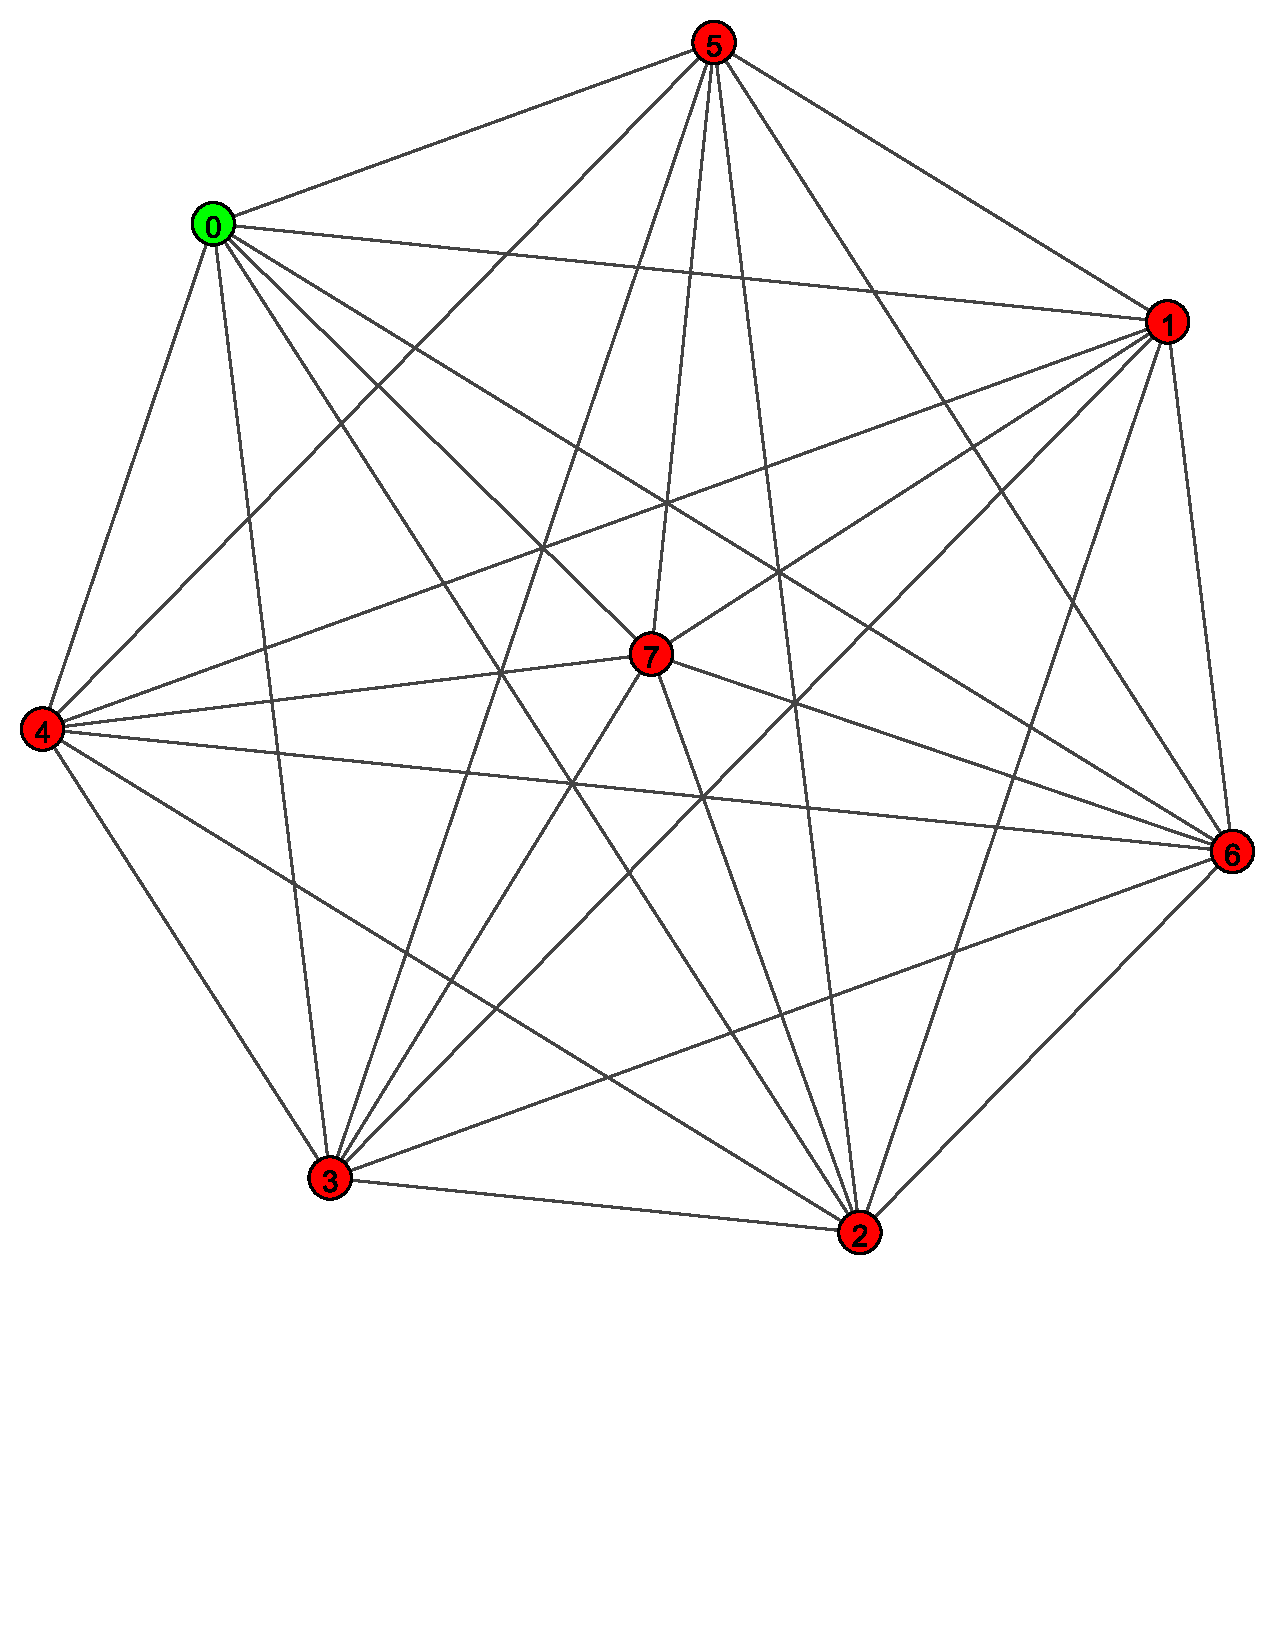
\includegraphics[width=5cm, trim = 0 6cm 0 0, clip]{images/graph_a.pdf}
\end{figure}

\begin{figure}[H]
    \centering
    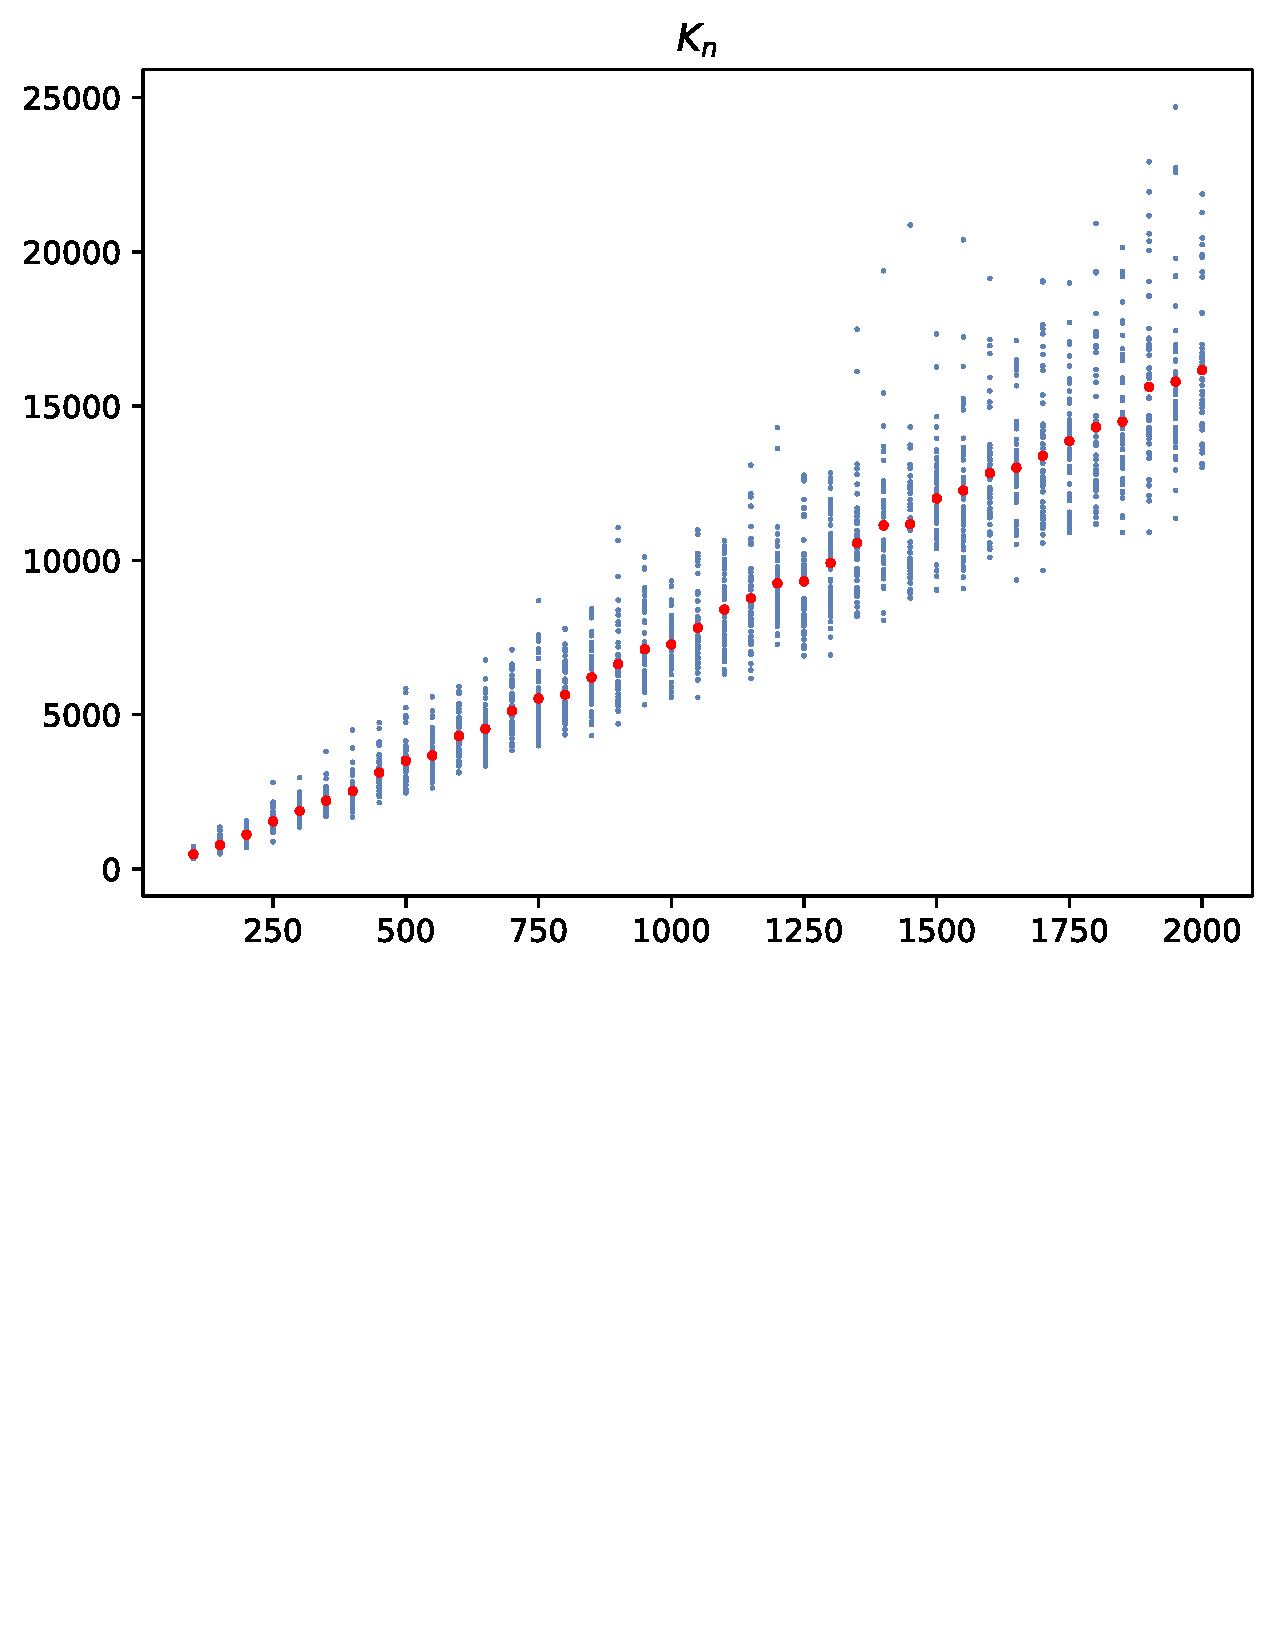
\includegraphics[width=12cm, trim = 0 11cm 0 0, clip]{images/a.pdf}
\end{figure}

\begin{figure}[H]
    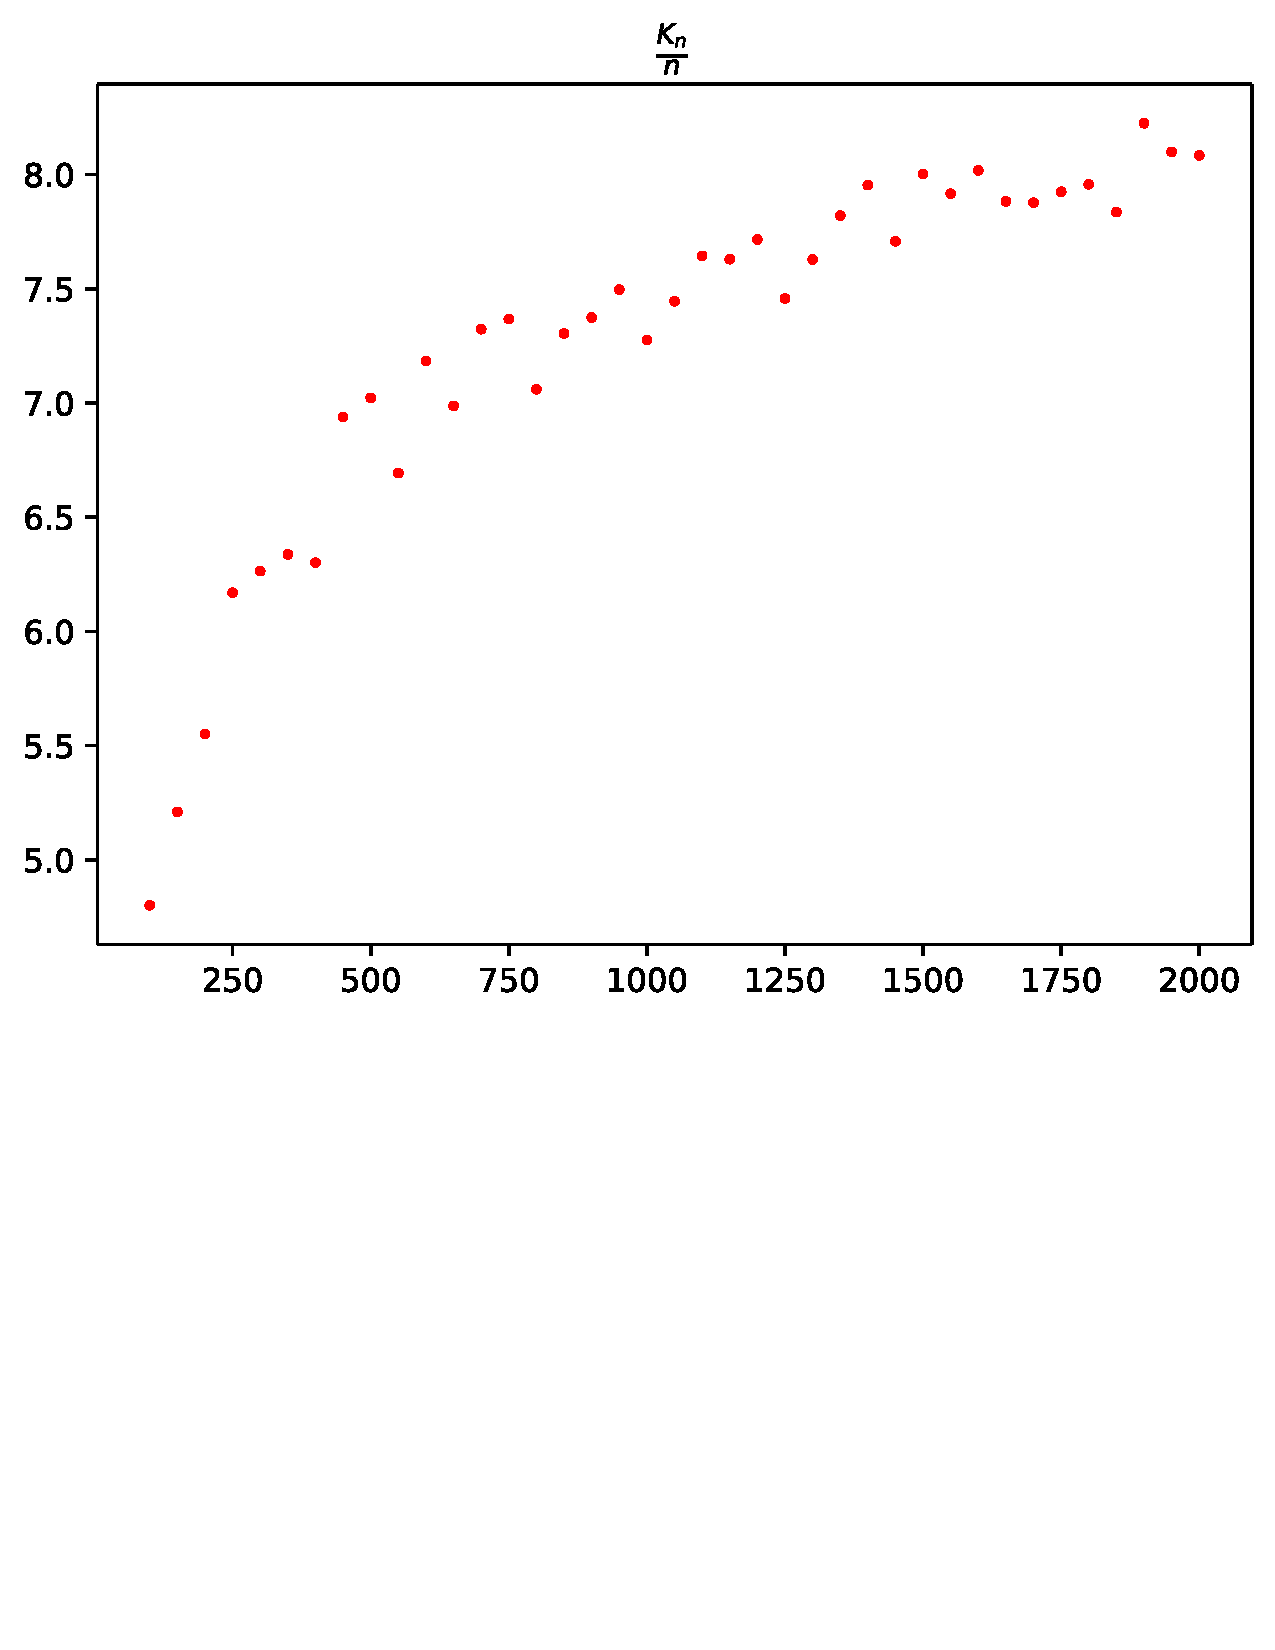
\includegraphics[width=8cm, trim = 0 11cm 0 0, clip]{images/a1.pdf}
    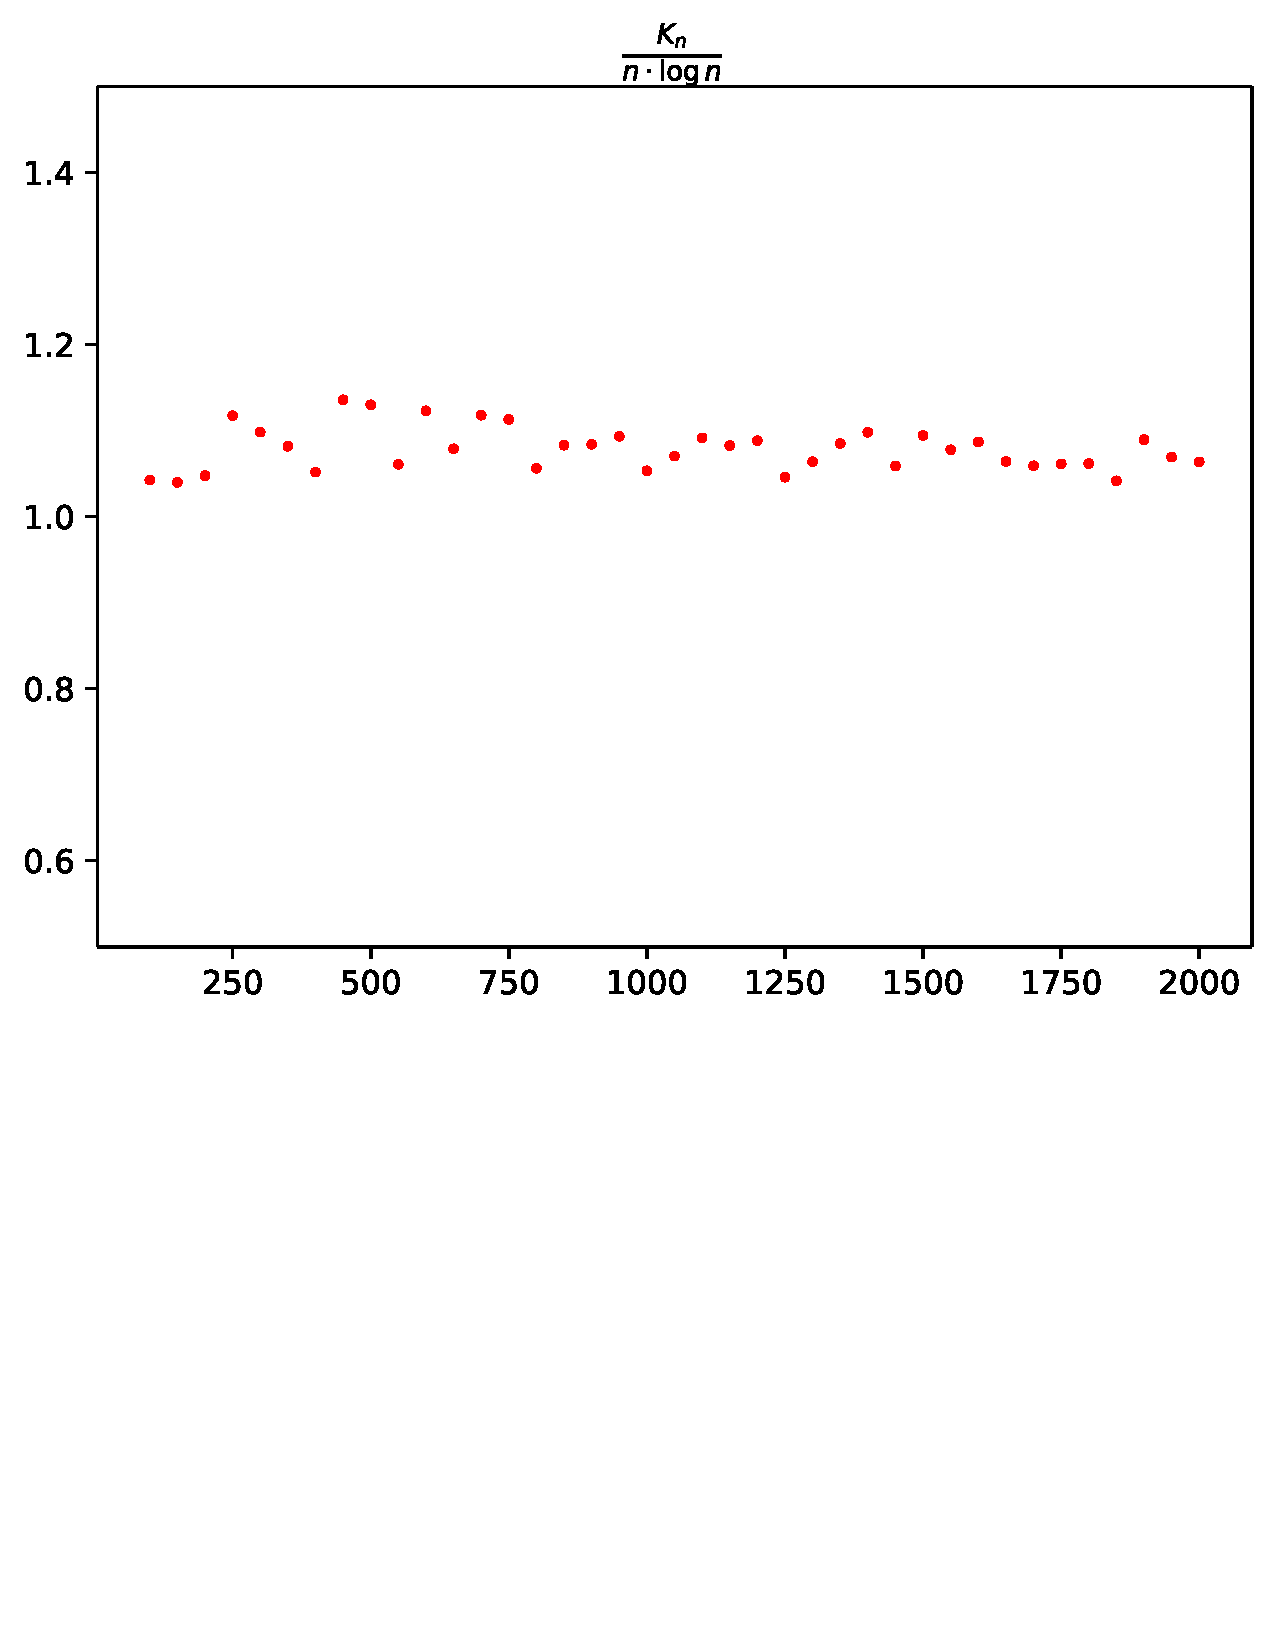
\includegraphics[width=8cm, trim = 0 11cm 0 0, clip]{images/a2.pdf}
\end{figure}

Na początku mogłoby się wydawać, że $K_n$ rośnie liniowo. Jednak pierwszy z mniejszych wykresów temu przeczy. Za to drugi wykres pozwala postawić hipotezę, iż
\[ K_n = \Theta (n \cdot \log n). \]

\subsection{Ścieżka ($P_n$)}

\subsubsection{Start w środku ścieżki ($X_0 = \lfloor n/2 \rfloor$)}

\begin{figure}[H]
    \centering
    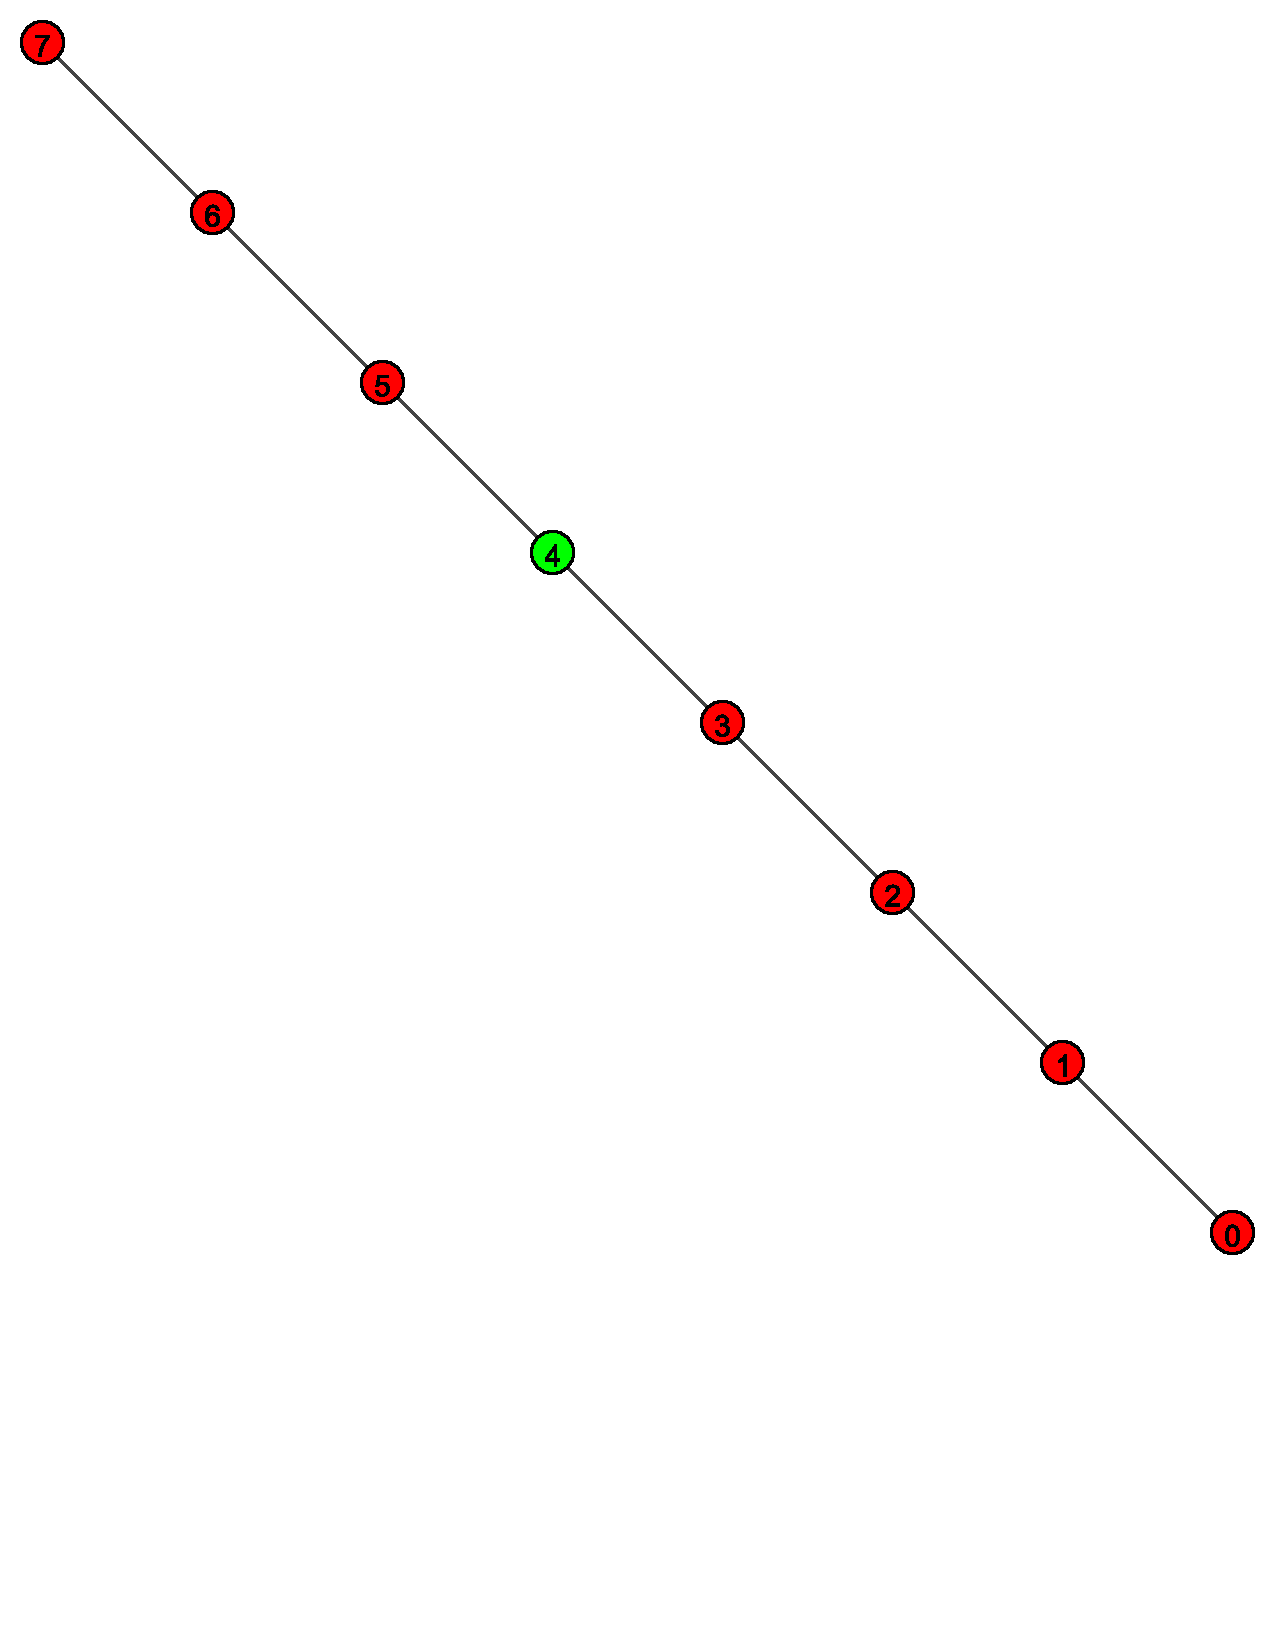
\includegraphics[width=5cm, trim = 0 6cm 0 0, clip]{images/graph_b.pdf}
\end{figure}

\begin{figure}[H]
    \centering
    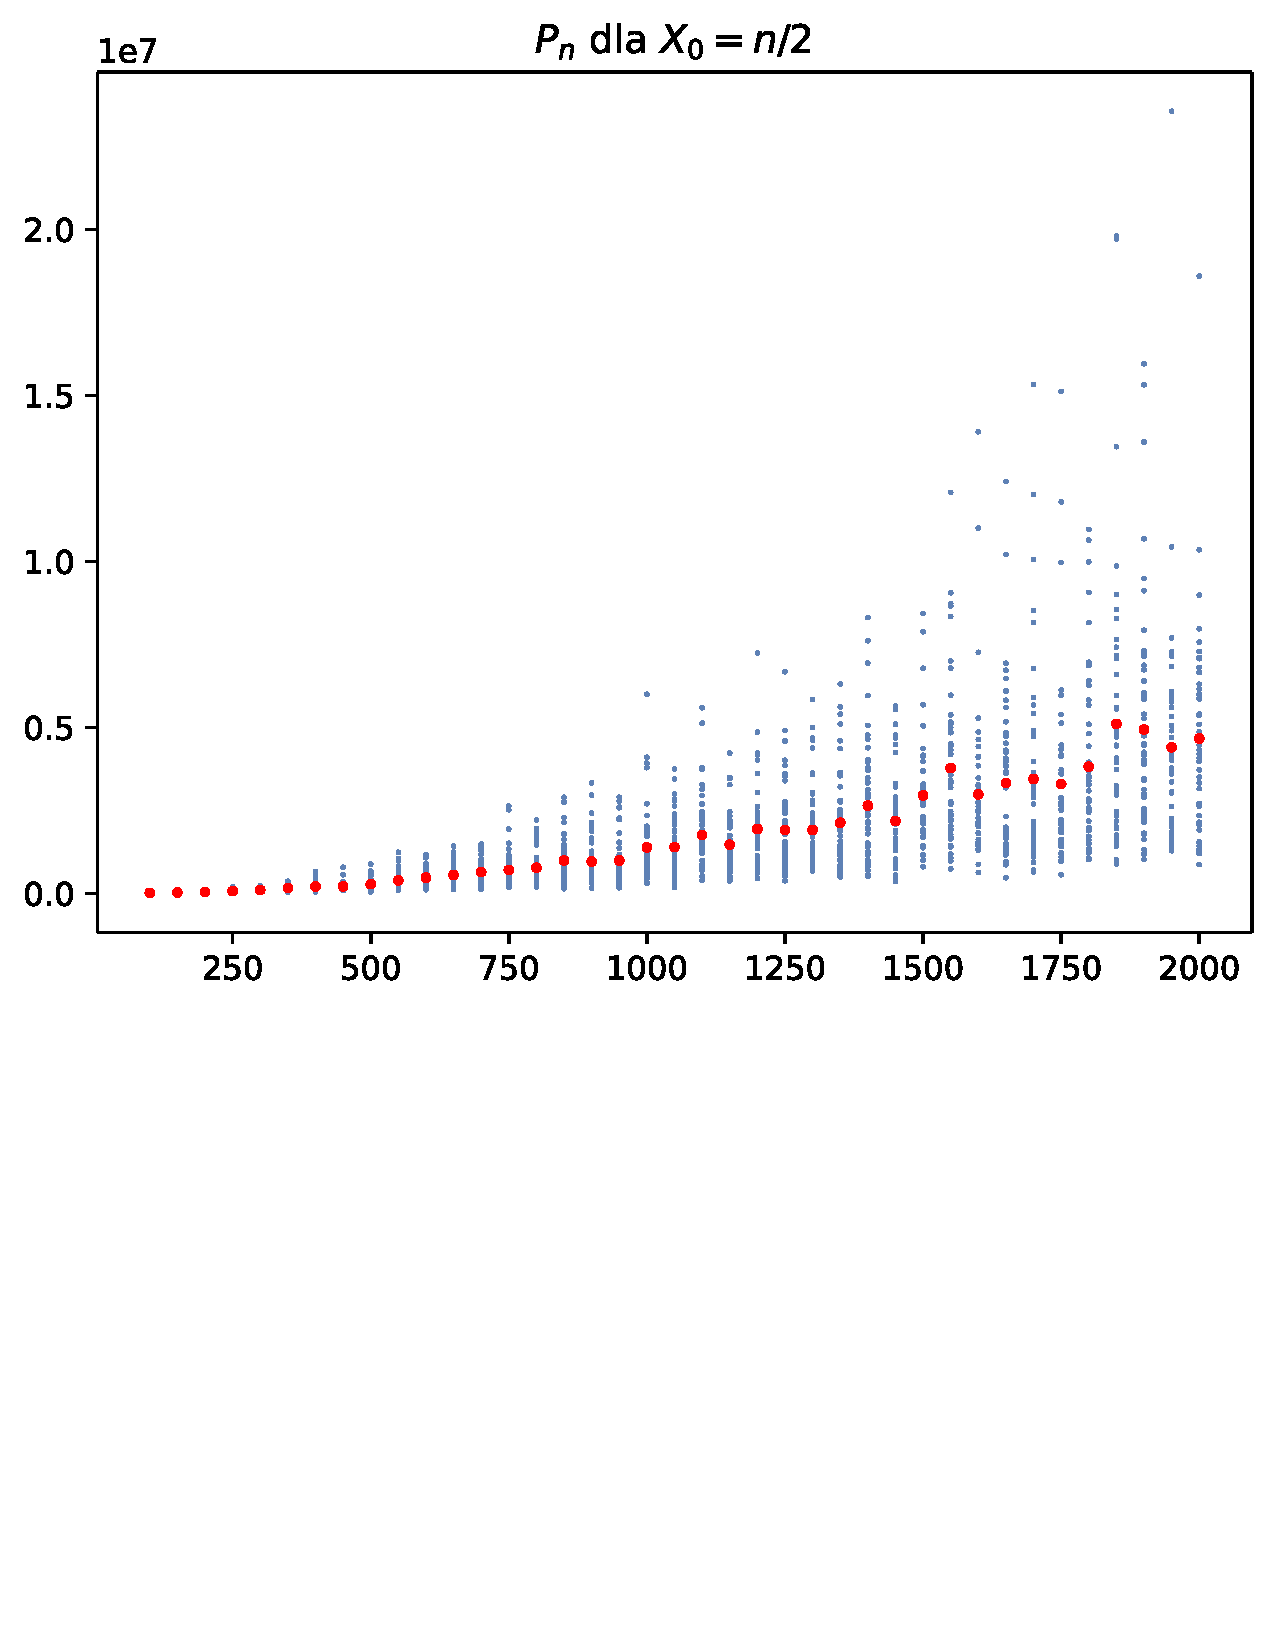
\includegraphics[width=12cm, trim = 0 11cm 0 0, clip]{images/b.pdf}
\end{figure}

\begin{figure}[H]
    \centering
    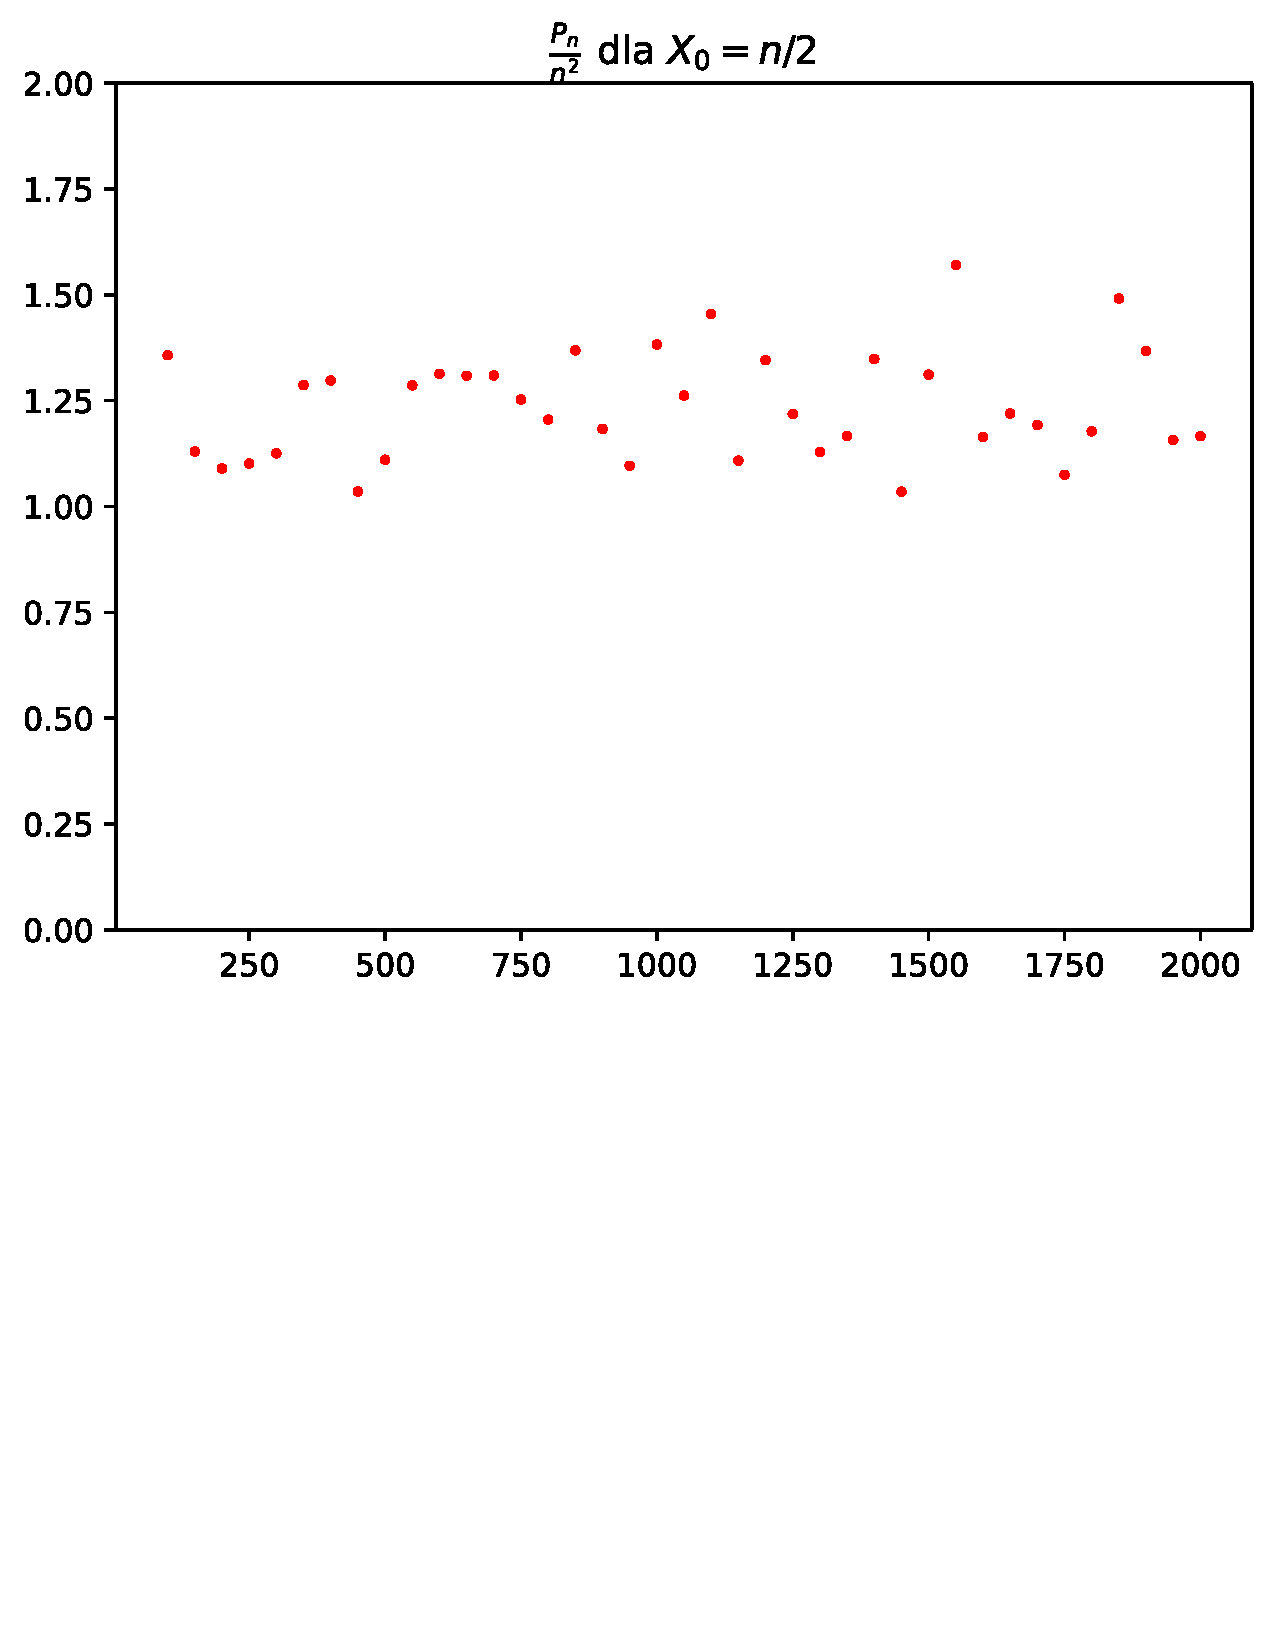
\includegraphics[width=12cm, trim = 0 11cm 0 0, clip]{images/b1.pdf}
\end{figure}

\subsubsection{Start na końcu ścieżki ($X_0 = 0$)}

\begin{figure}[H]
    \centering
    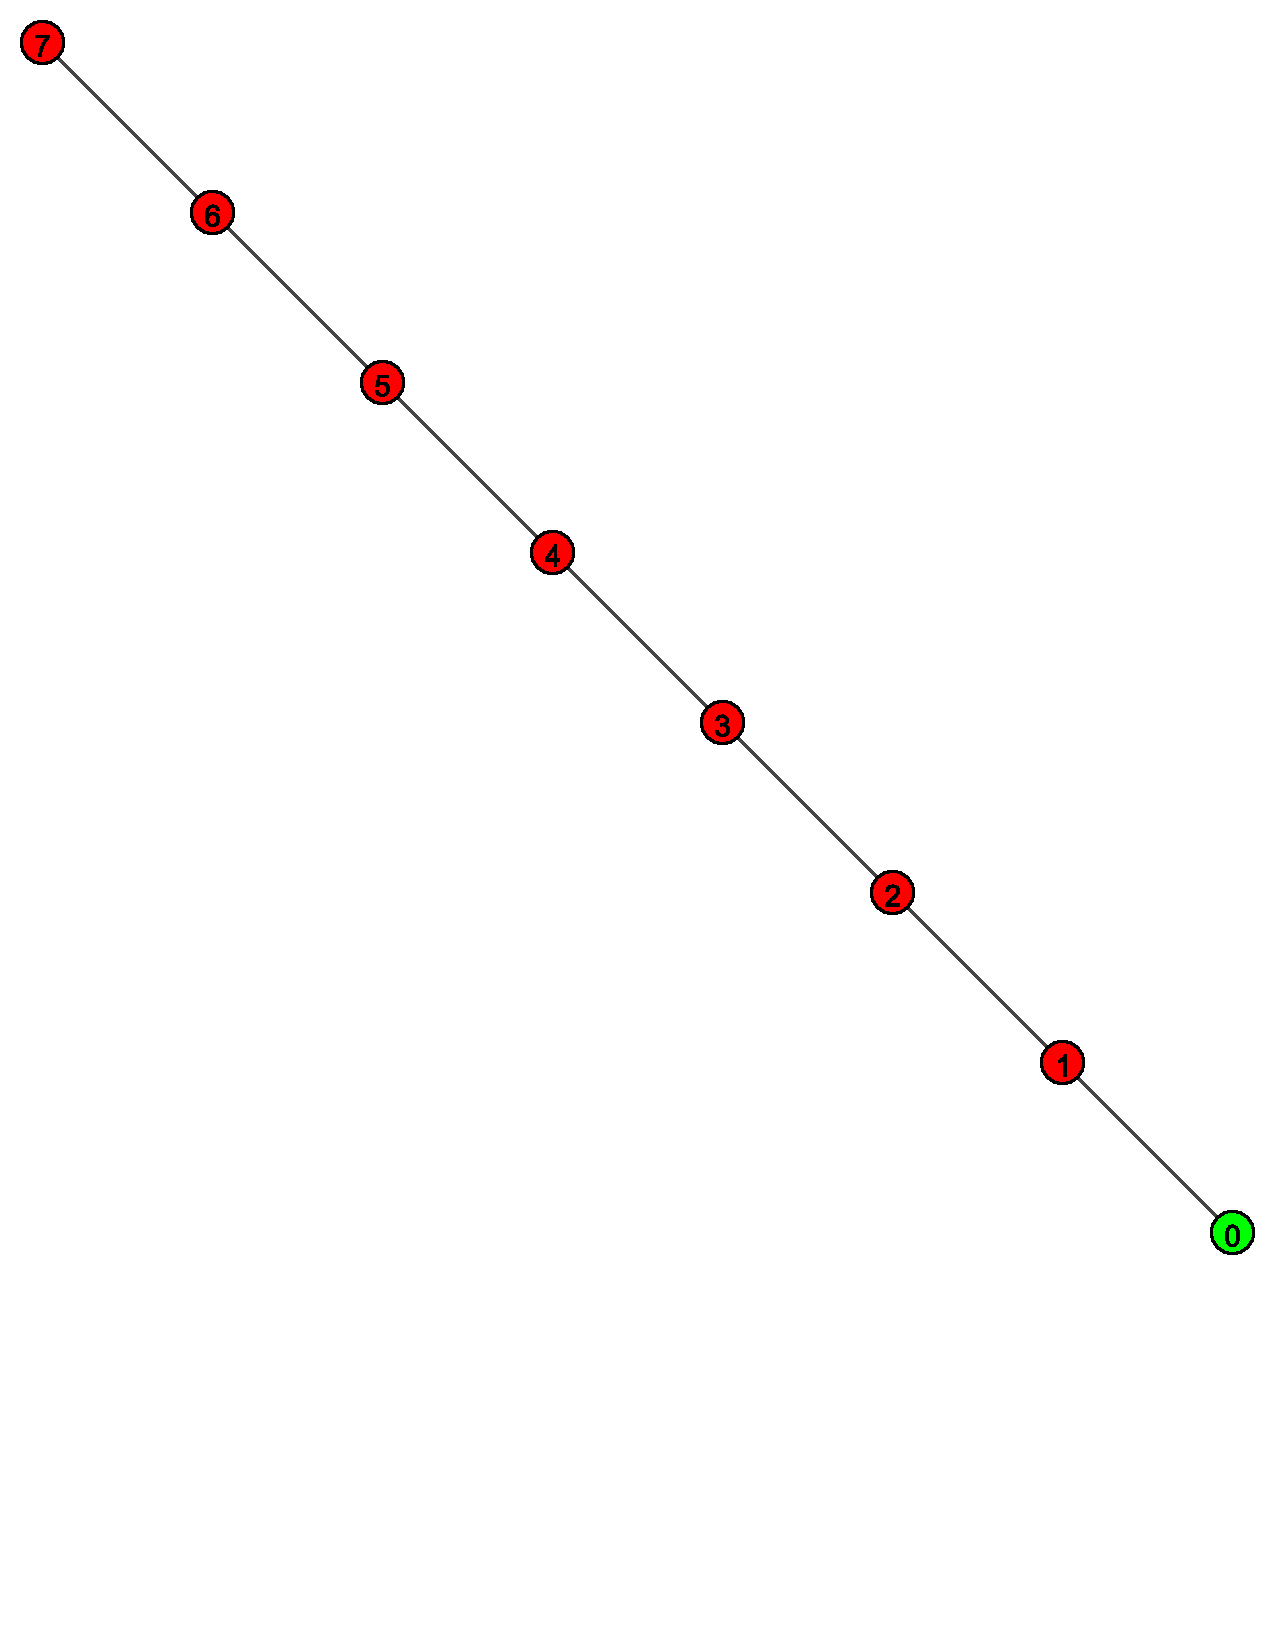
\includegraphics[width=5cm, trim = 0 6cm 0 0, clip]{images/graph_c.pdf}
\end{figure}

\begin{figure}[H]
    \centering
    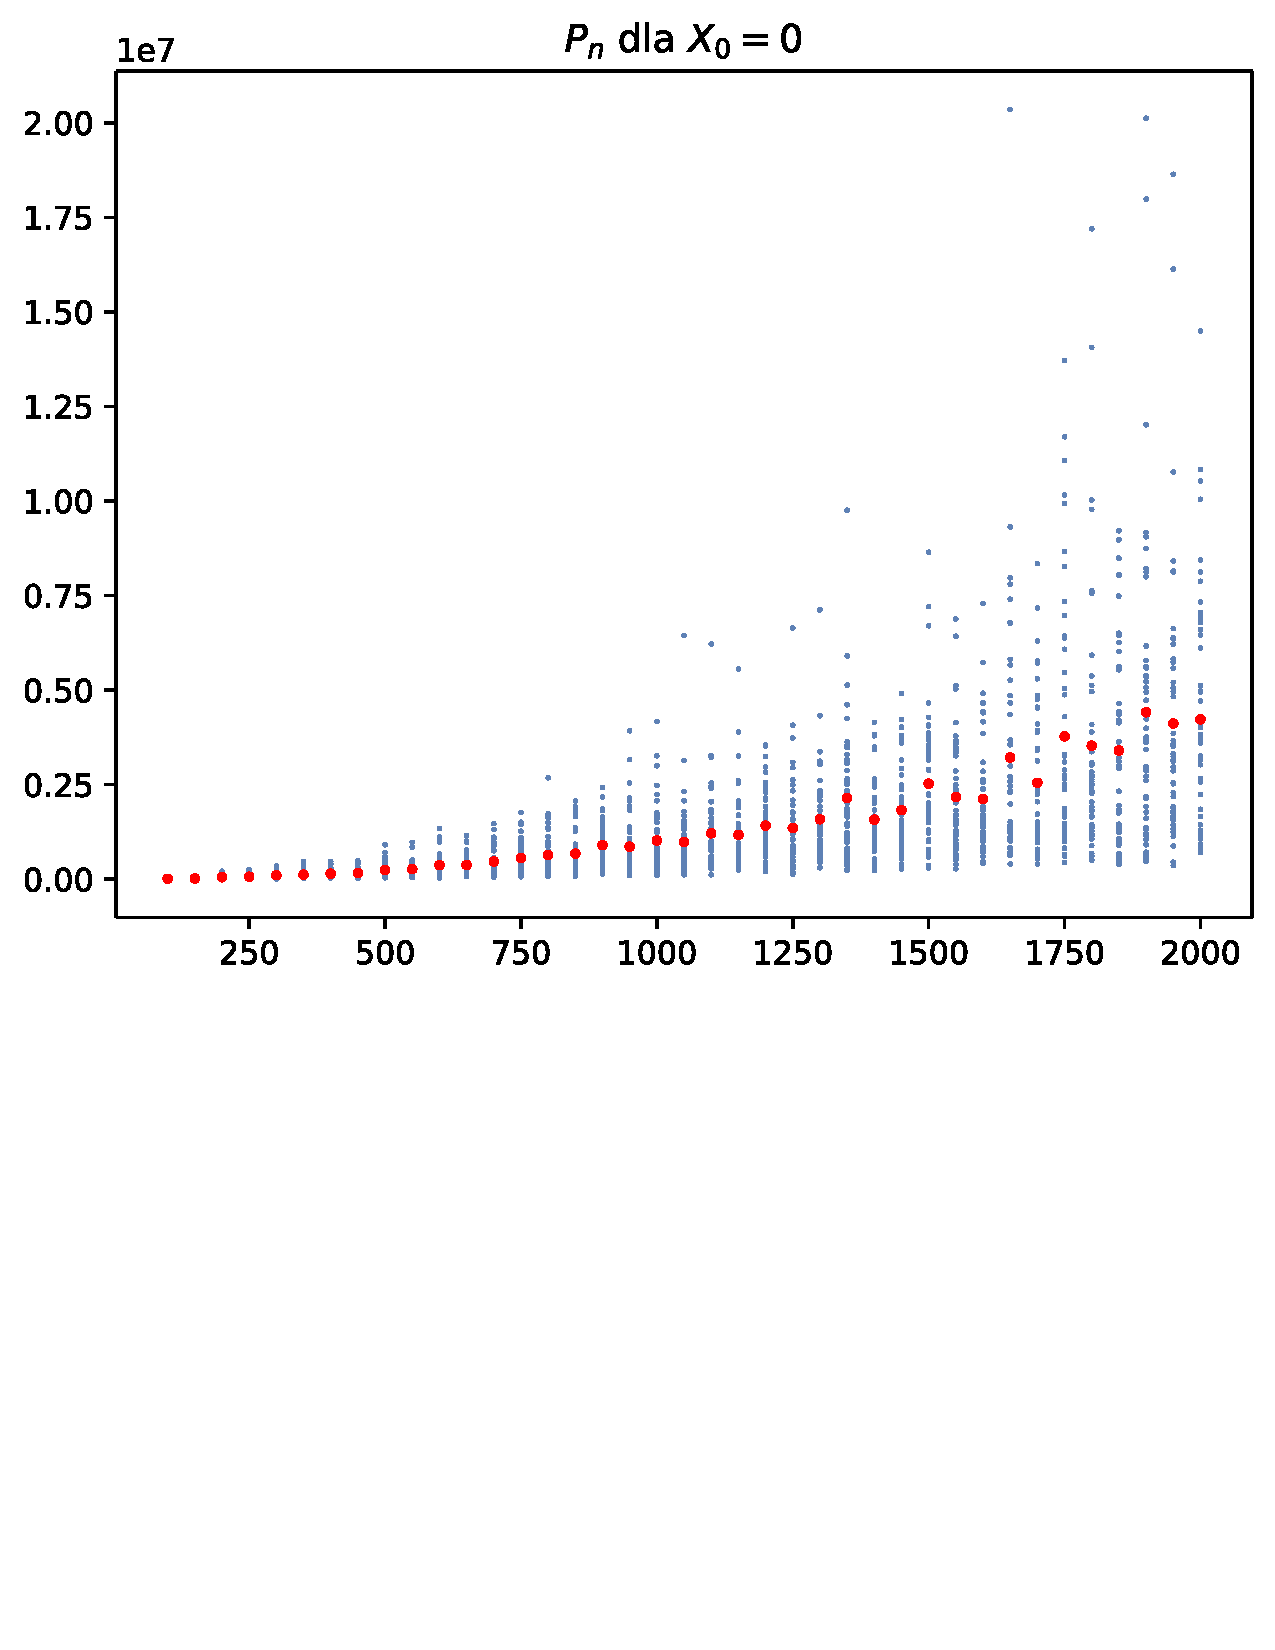
\includegraphics[width=12cm, trim = 0 11cm 0 0, clip]{images/c.pdf}
\end{figure}

\begin{figure}[H]
    \centering
    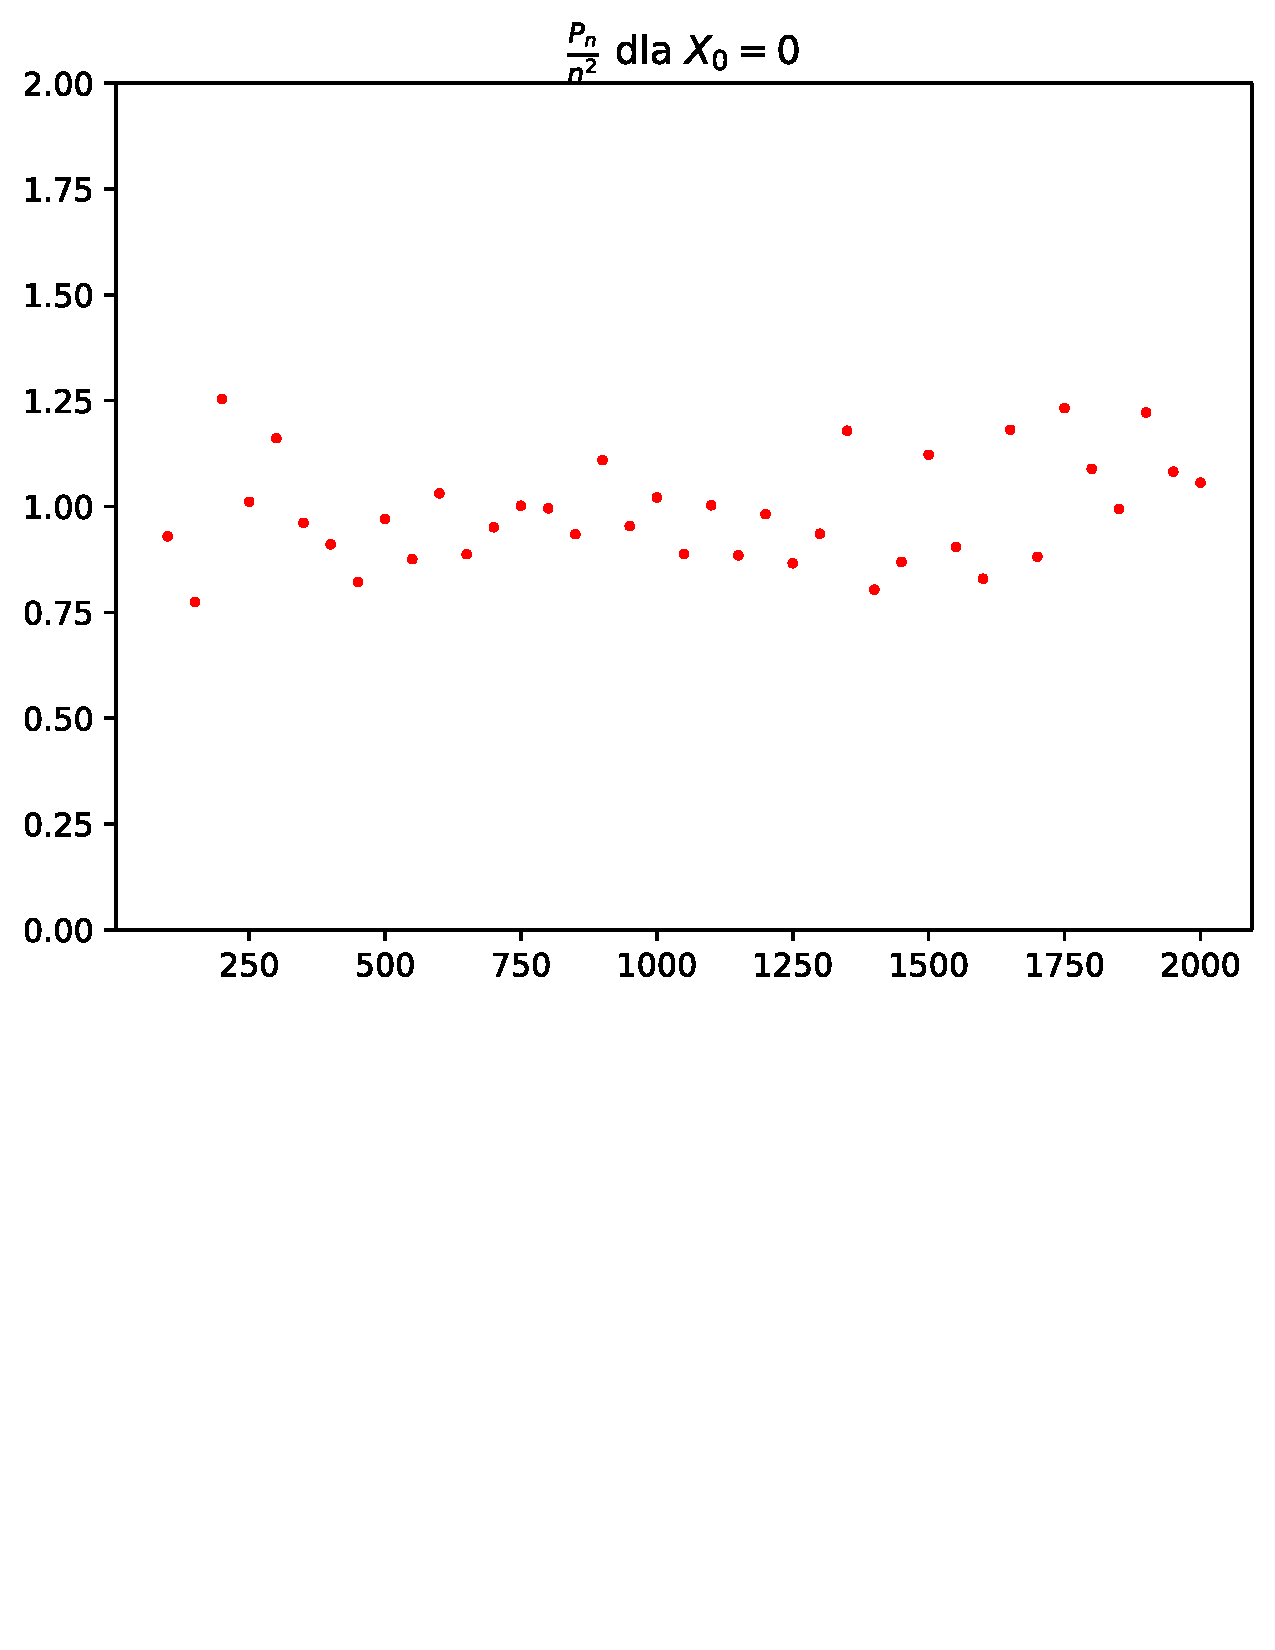
\includegraphics[width=12cm, trim = 0 11cm 0 0, clip]{images/c1.pdf}
\end{figure}

Jak widać na powyższych wykresach niezależnie od punktu startowego
\[ P_n = \Theta (n^2). \]
Jedyną różnicą jest to, że dla $X_0 = 0$ czas pokrycia jest krótszy. Prawdopodobnie wynika to  z tego, że prawdopodobieństwo znalezienia się na końcu ścieżki jest małe, a zaczynając na jej końcu już jeden z nich został odwiedzony.

\subsection{Zupełne drzewo binarne ($T_n$)}

\begin{figure}[H]
    \centering
    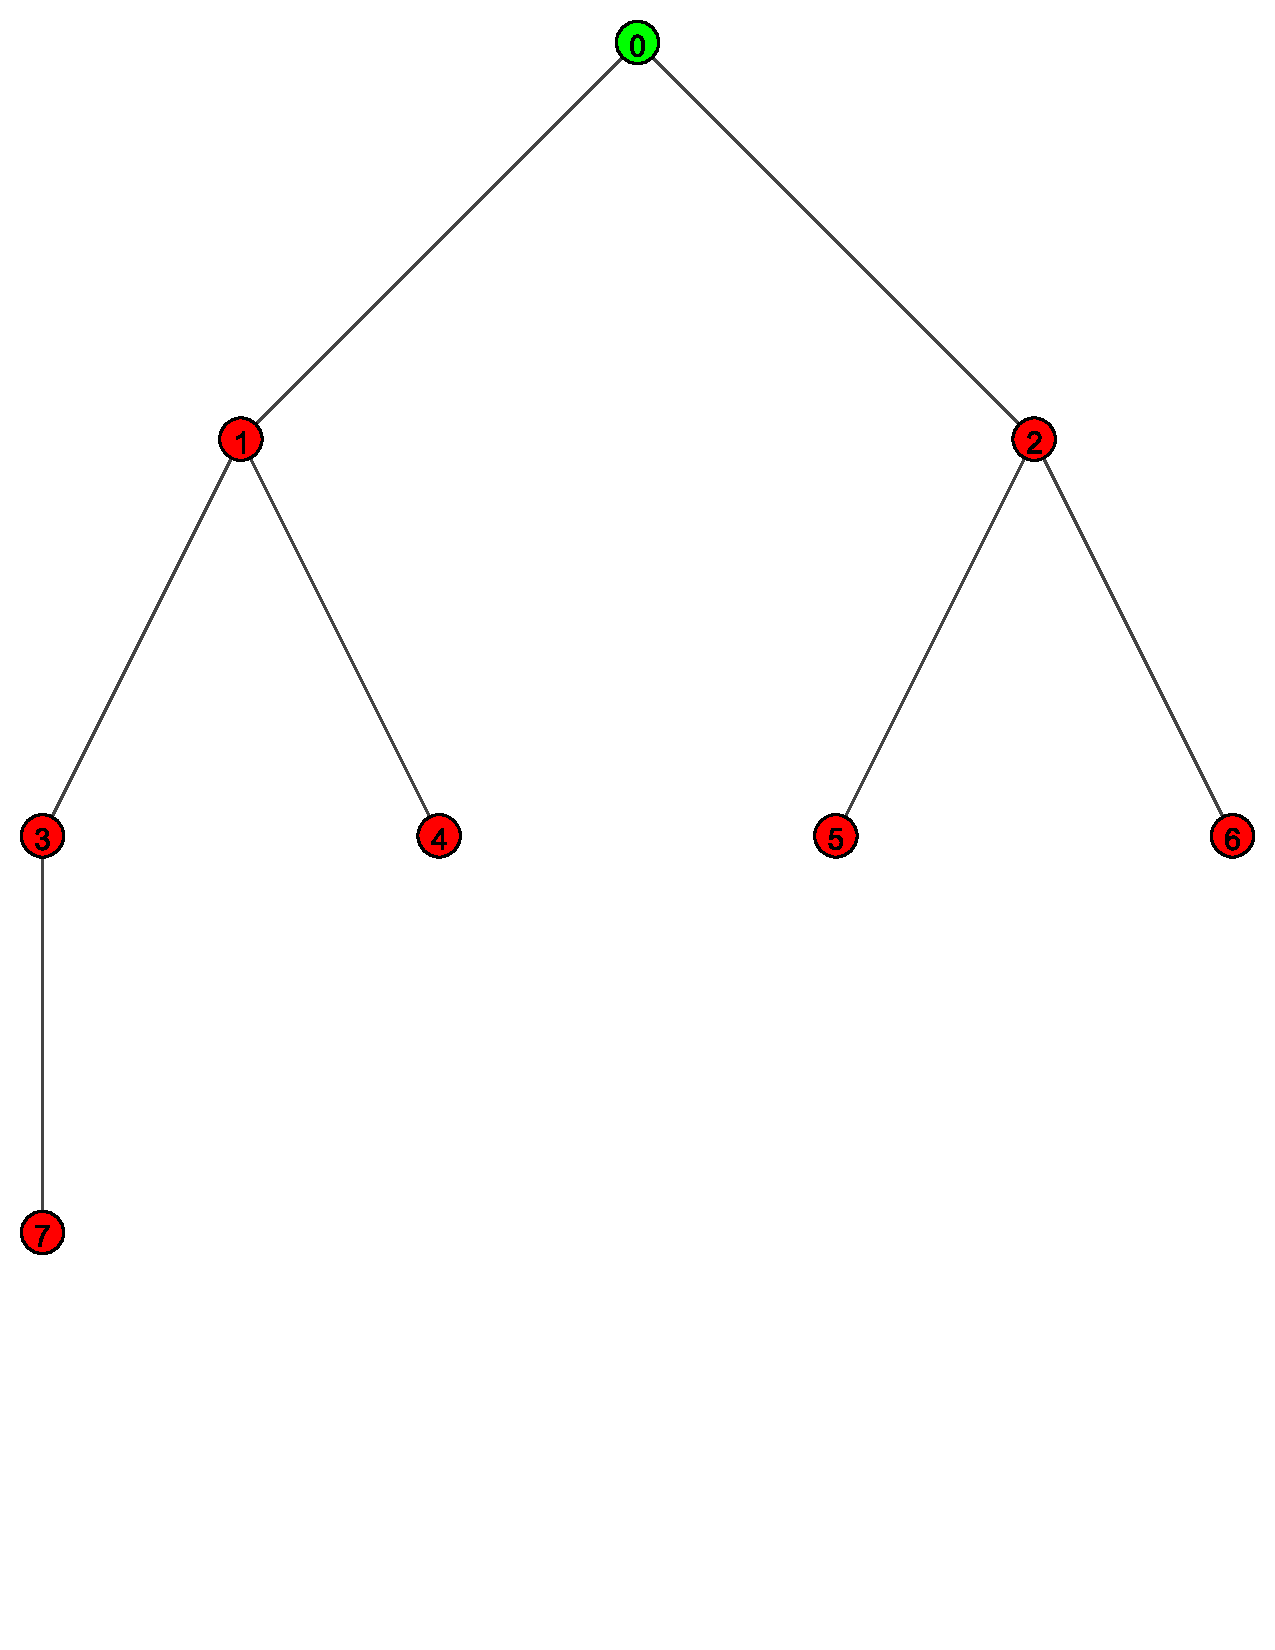
\includegraphics[width=5cm, trim = 0 6cm 0 0, clip]{images/graph_d.pdf}
\end{figure}

\begin{figure}[H]
    \centering
    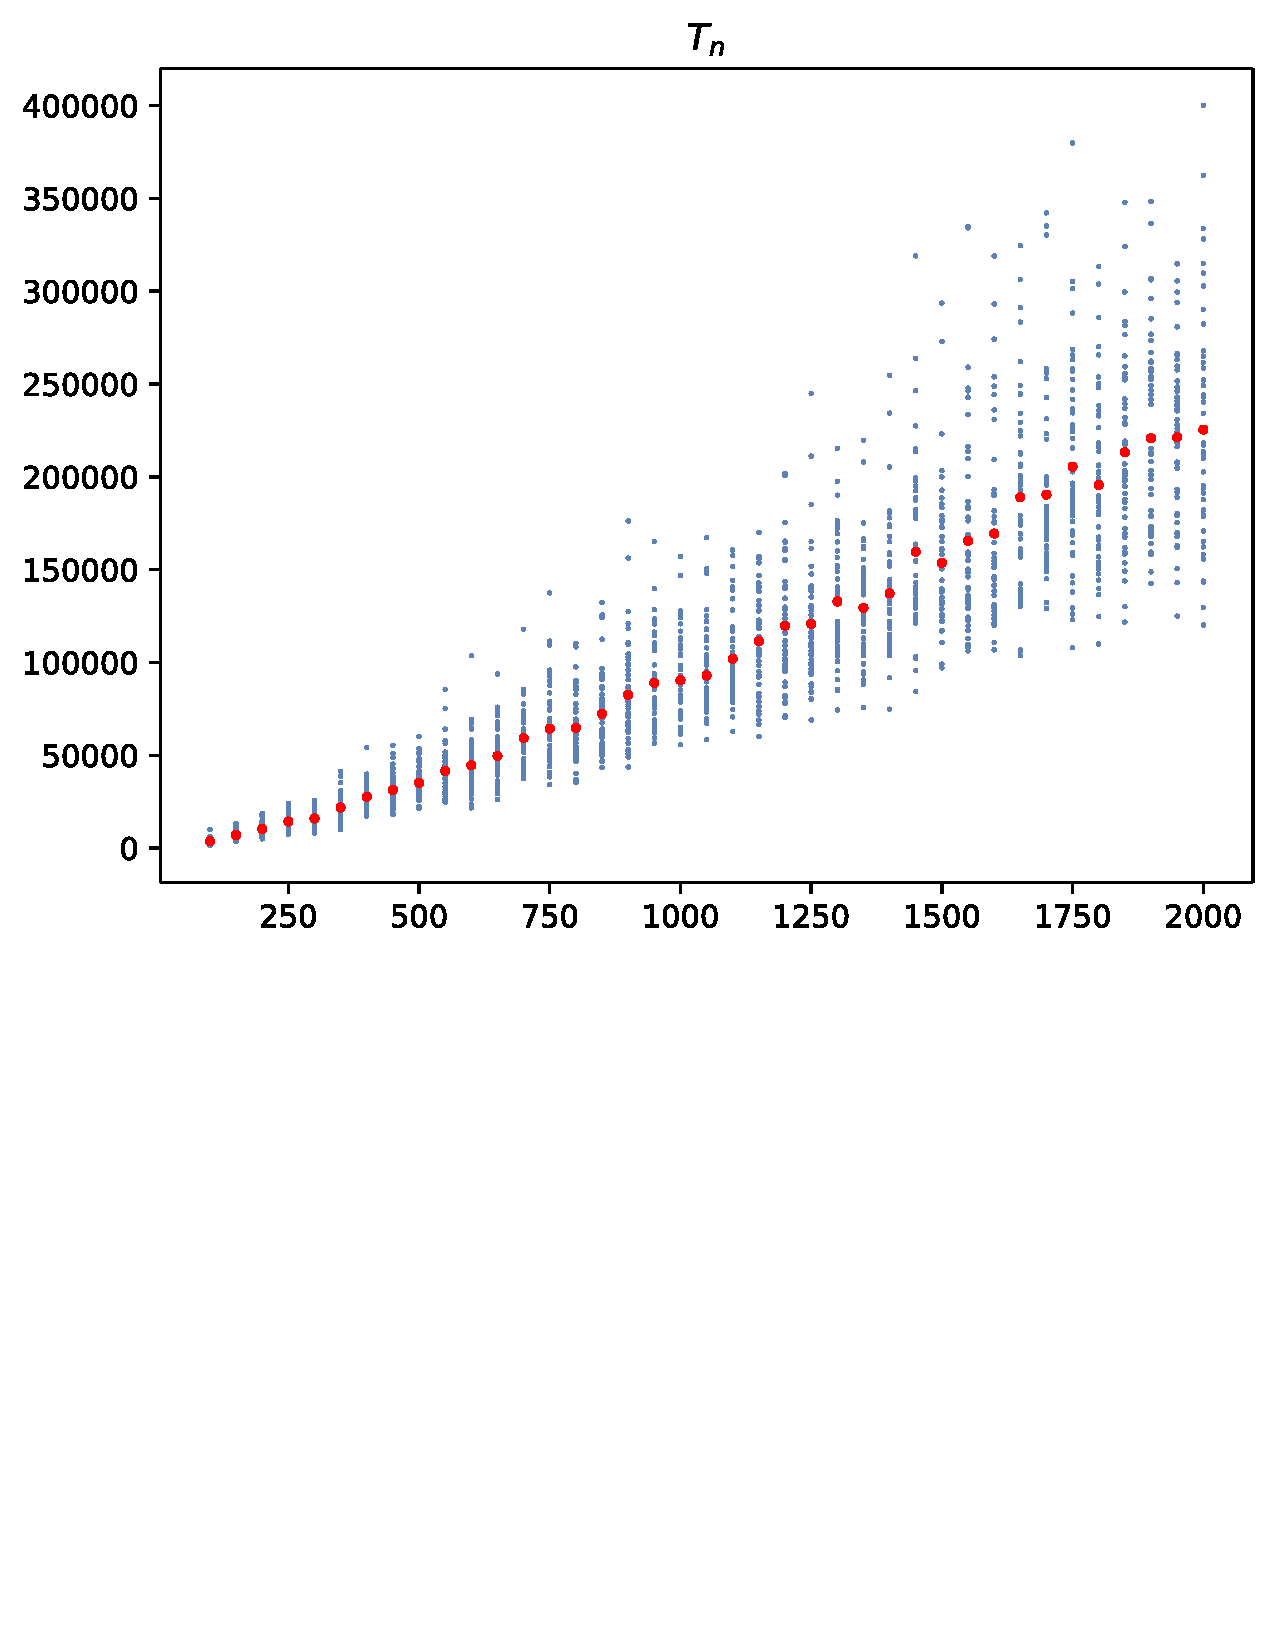
\includegraphics[width=12cm, trim = 0 11cm 0 0, clip]{images/d.pdf}
\end{figure}

\begin{figure}[H]
    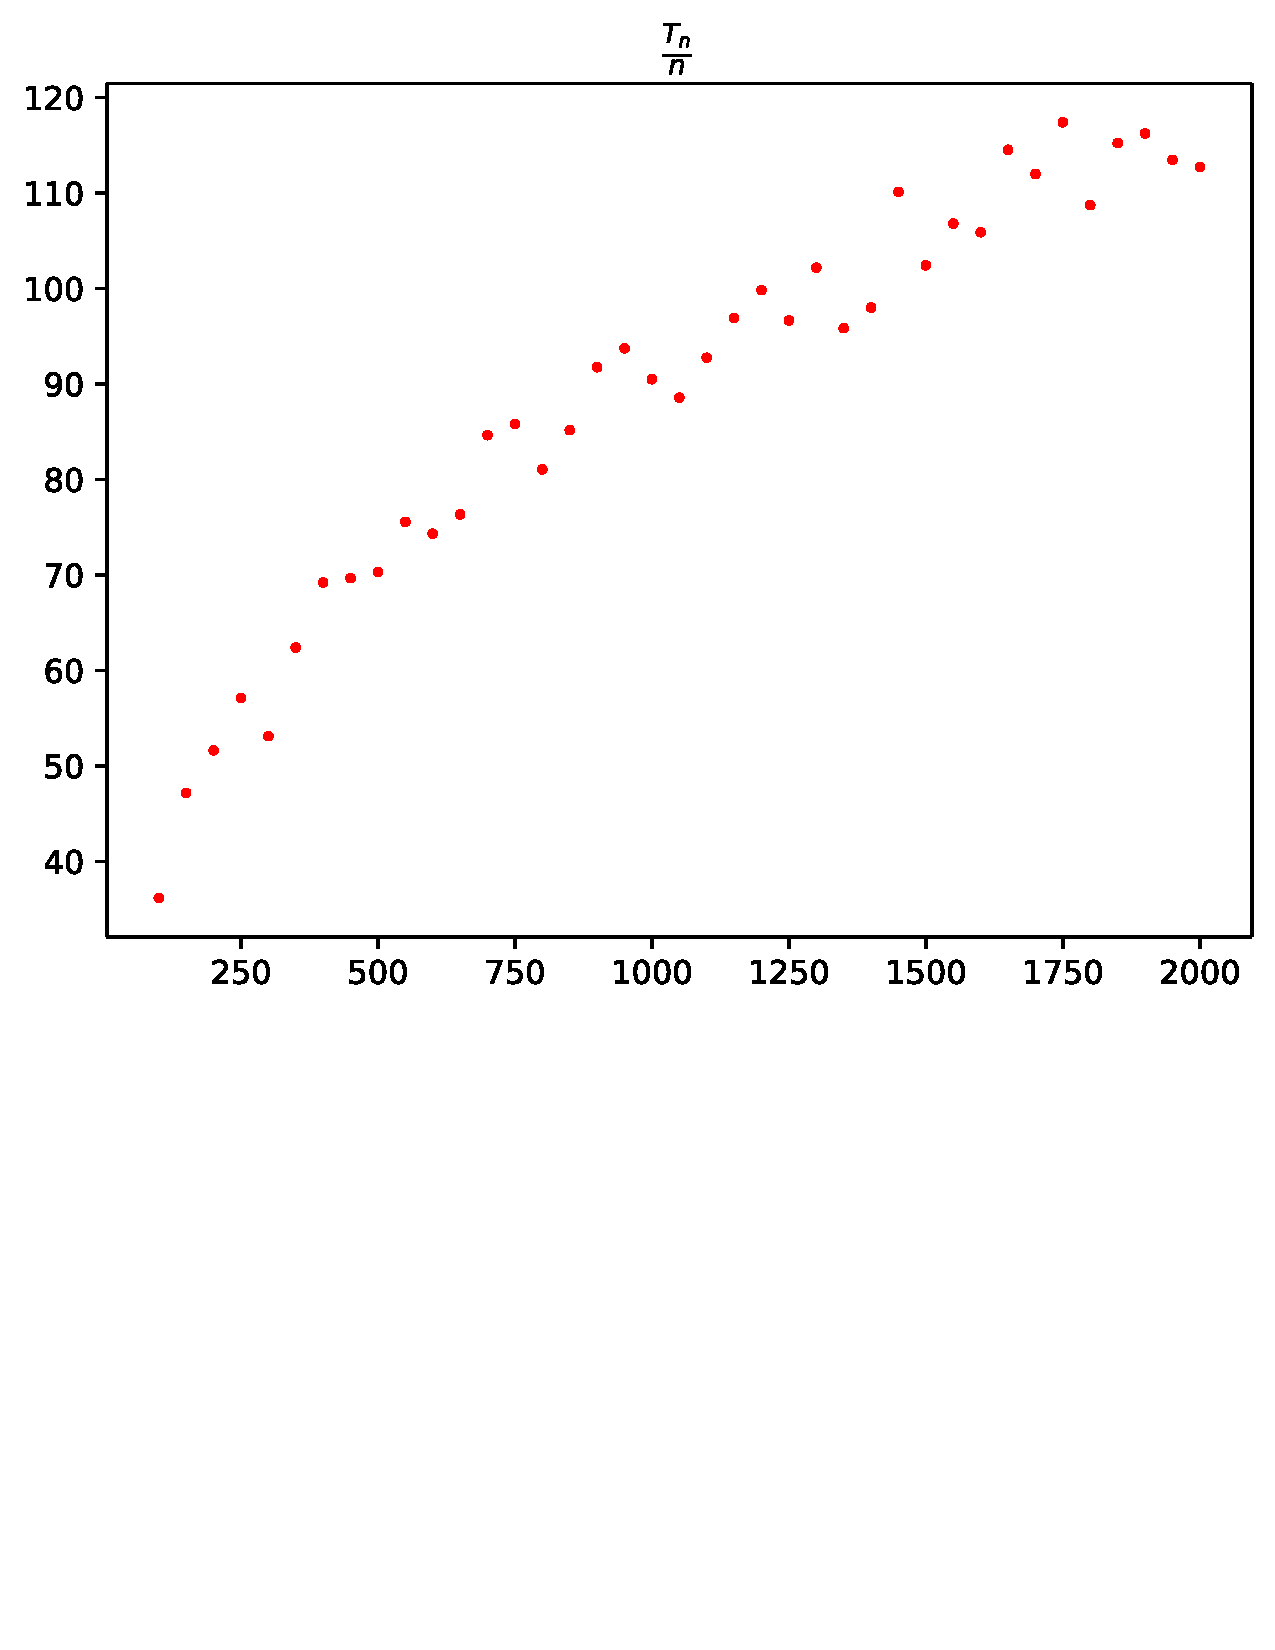
\includegraphics[width=8cm, trim = 0 11cm 0 0, clip]{images/d1.pdf}
    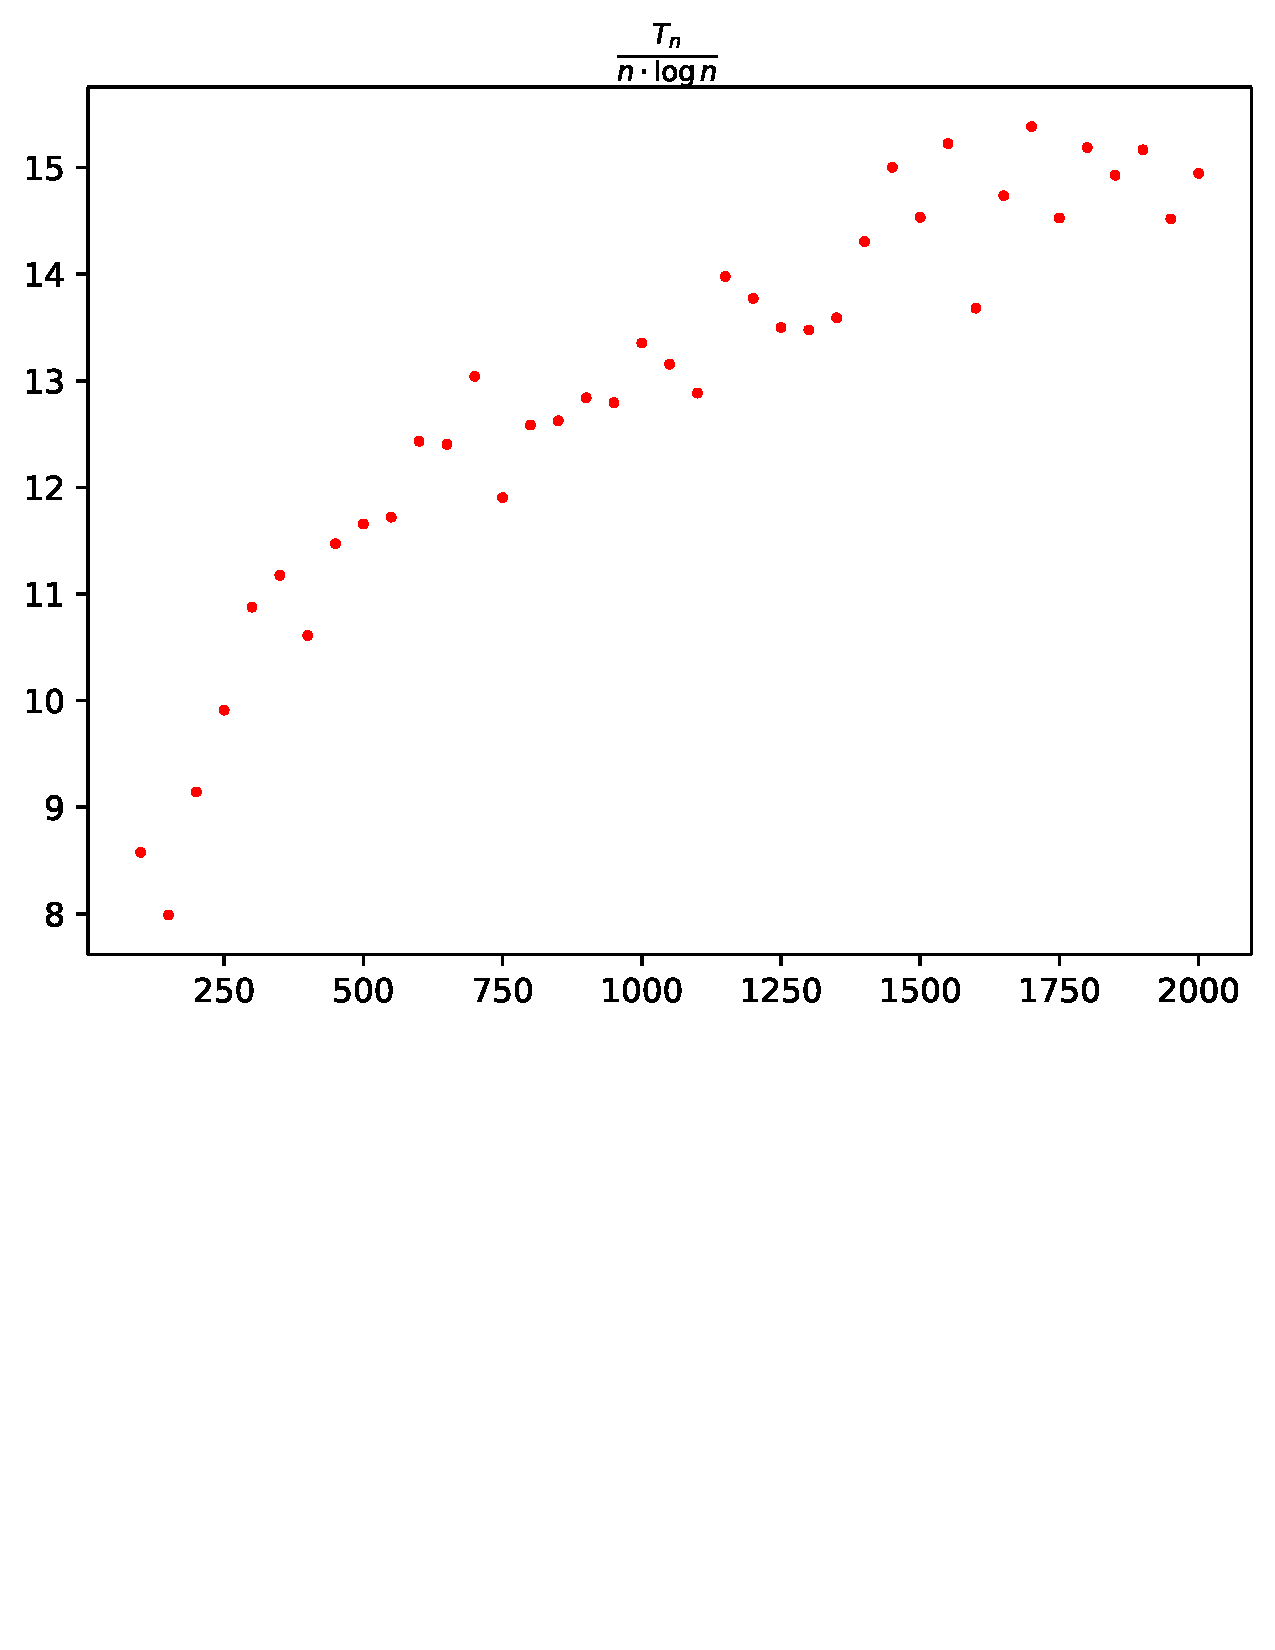
\includegraphics[width=8cm, trim = 0 11cm 0 0, clip]{images/d3.pdf}
\end{figure}

\begin{figure}[H]
    \centering
    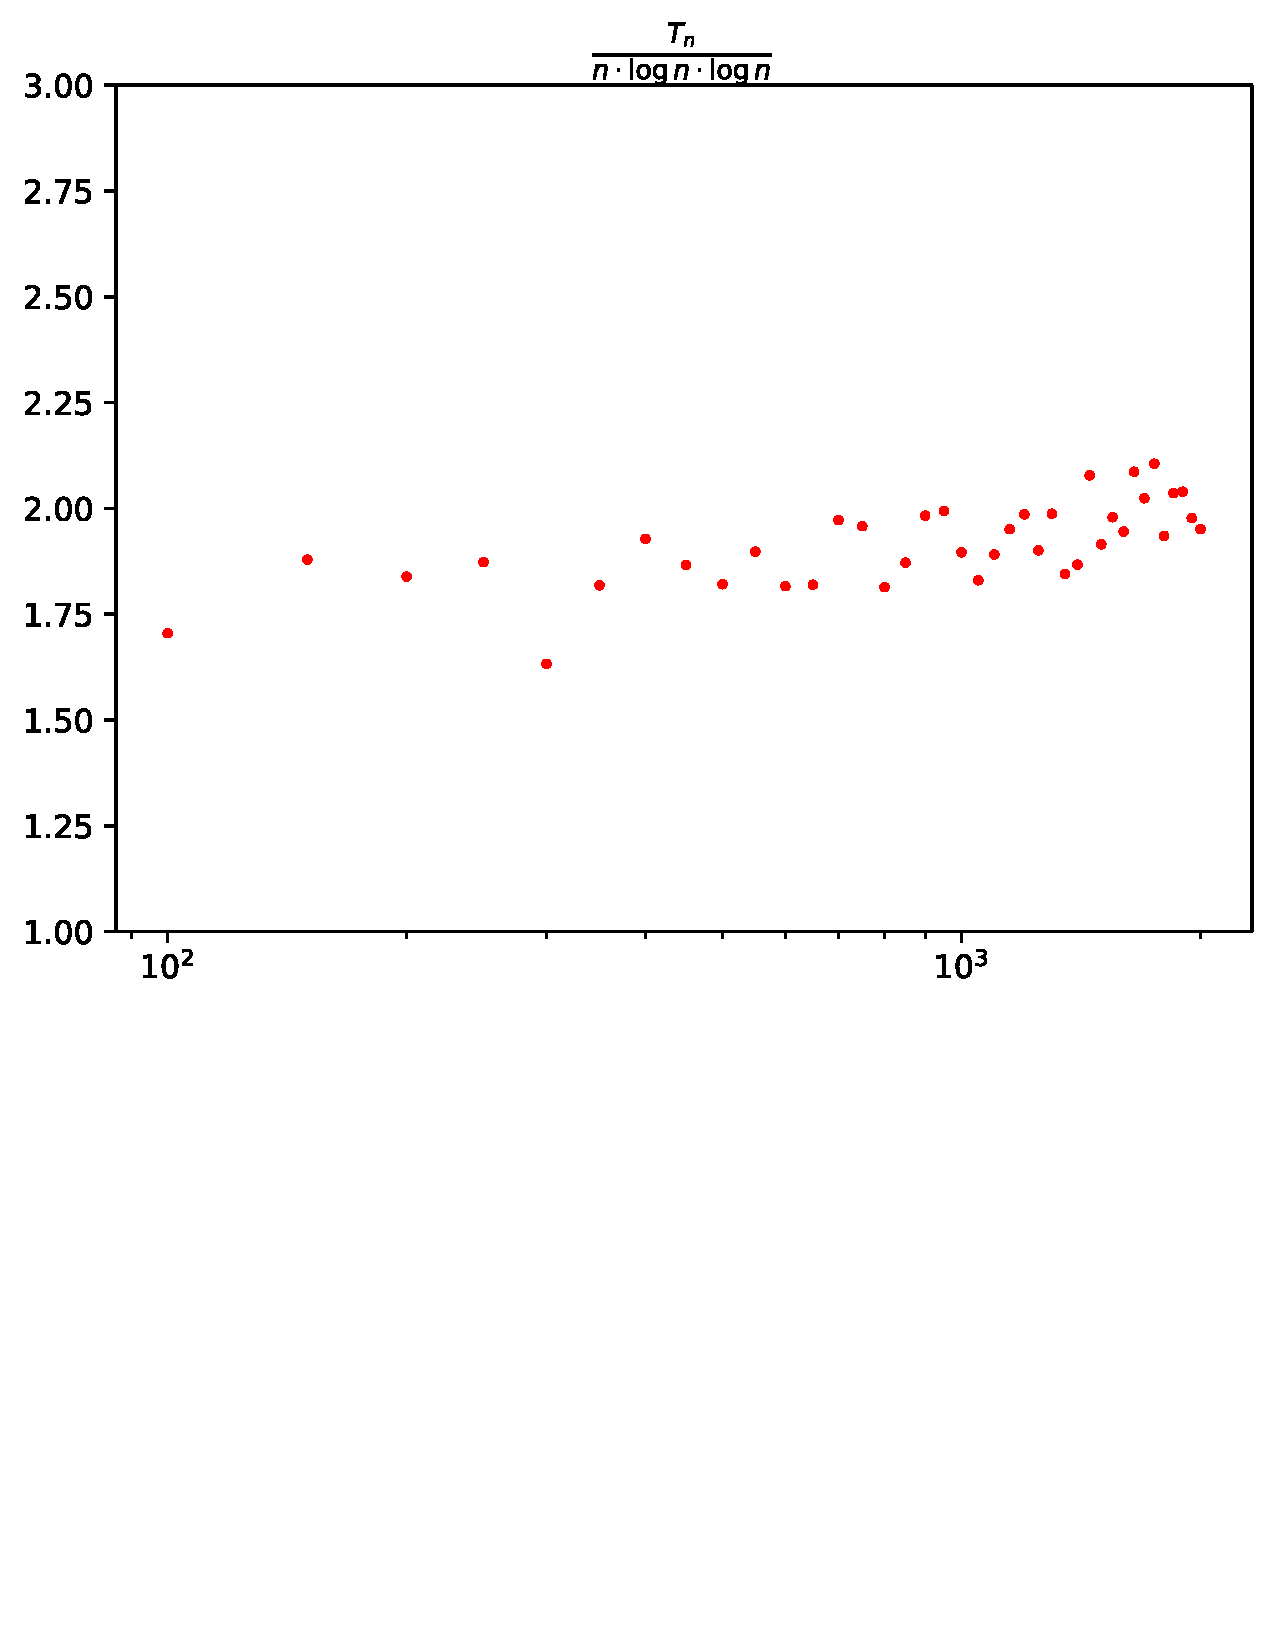
\includegraphics[width=12cm, trim = 0 11cm 0 0, clip]{images/d2.pdf}
\end{figure}

Wielkość $T_n$ wydaje się rosnąć liniowo, jednak nie potwierdza tego pierwszy z mniejszych wykresów. Nie jest to także $n \cdot \log n$. Po paru próbach doszedłem do wniosku, iż
\[ T_n = \Theta (n \cdot \log n \cdot \log n), \]
co potwierdza ostatni wykres.

\subsection{Lizak ($L_n$)}

\begin{figure}[H]
    \centering
    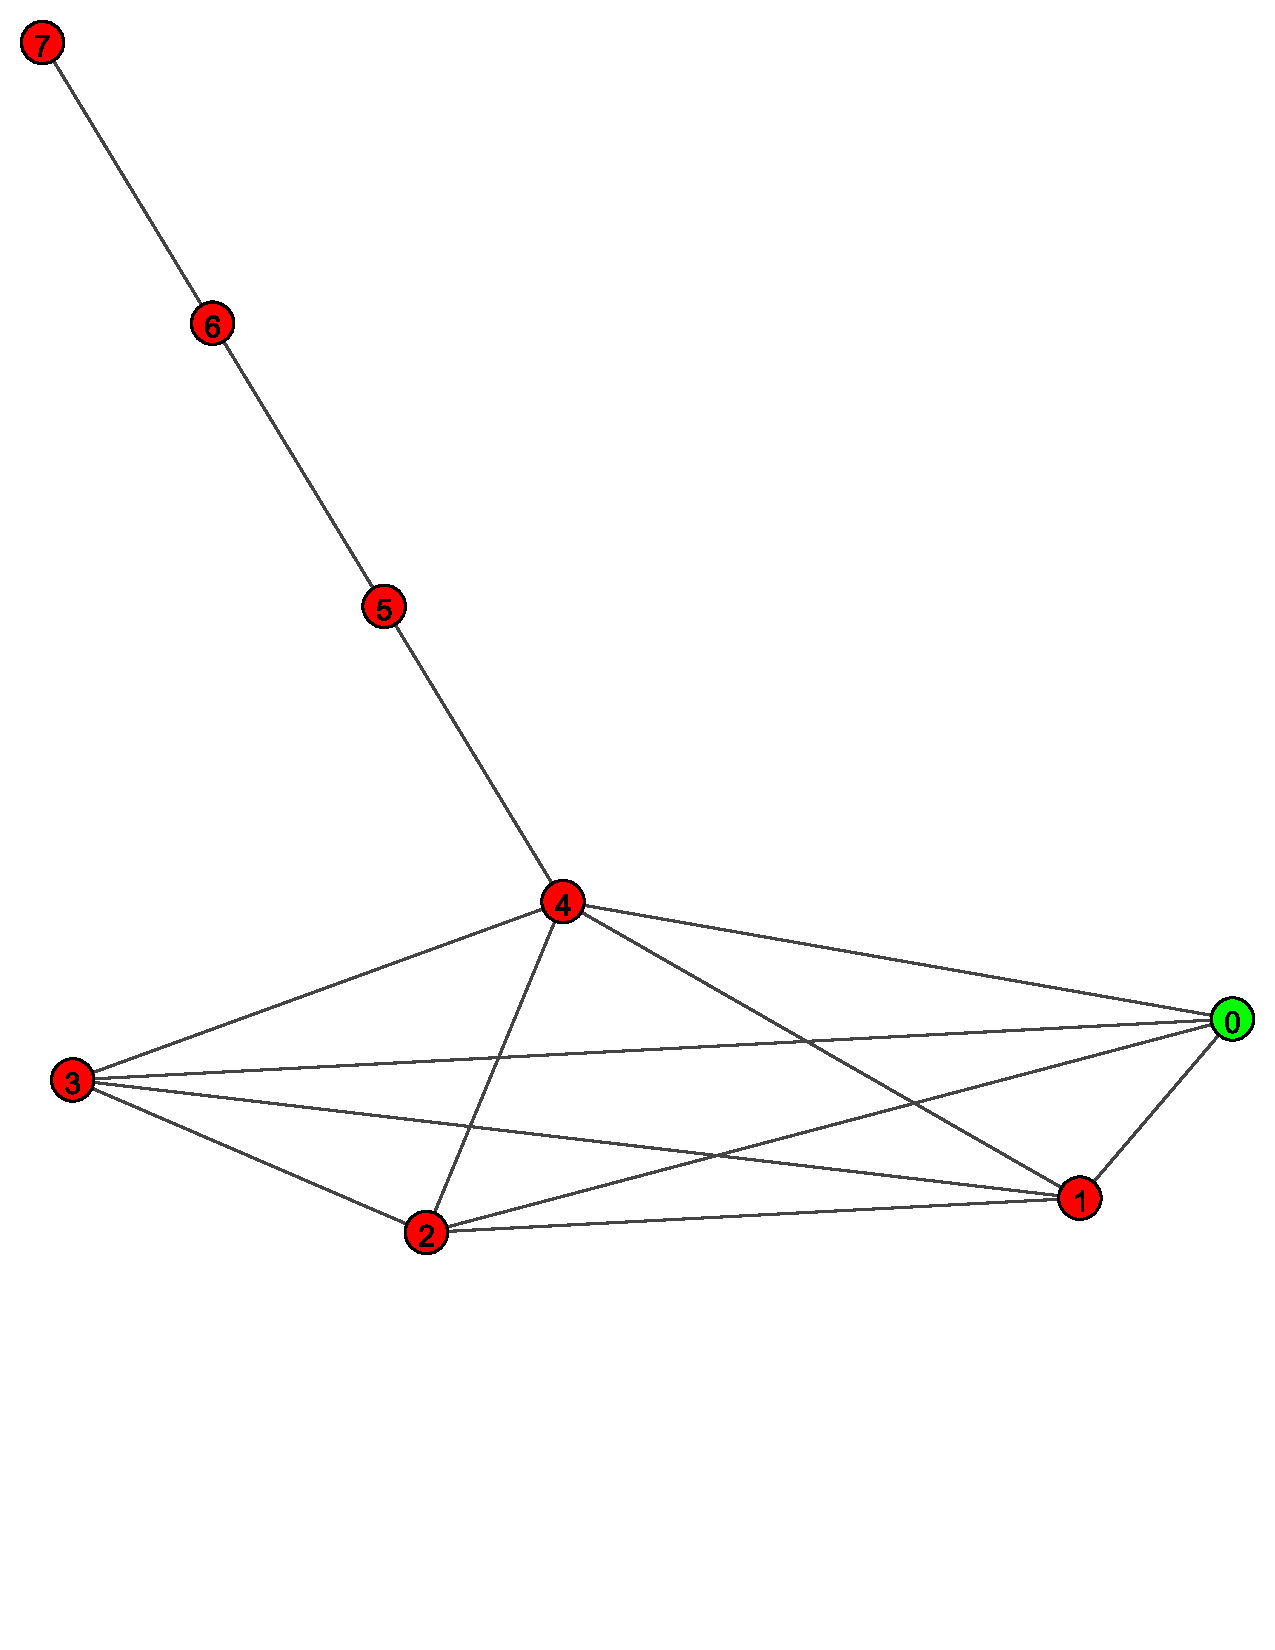
\includegraphics[width=5cm, trim = 0 6cm 0 0, clip]{images/graph_e.pdf}
\end{figure}

\begin{figure}[H]
    \centering
    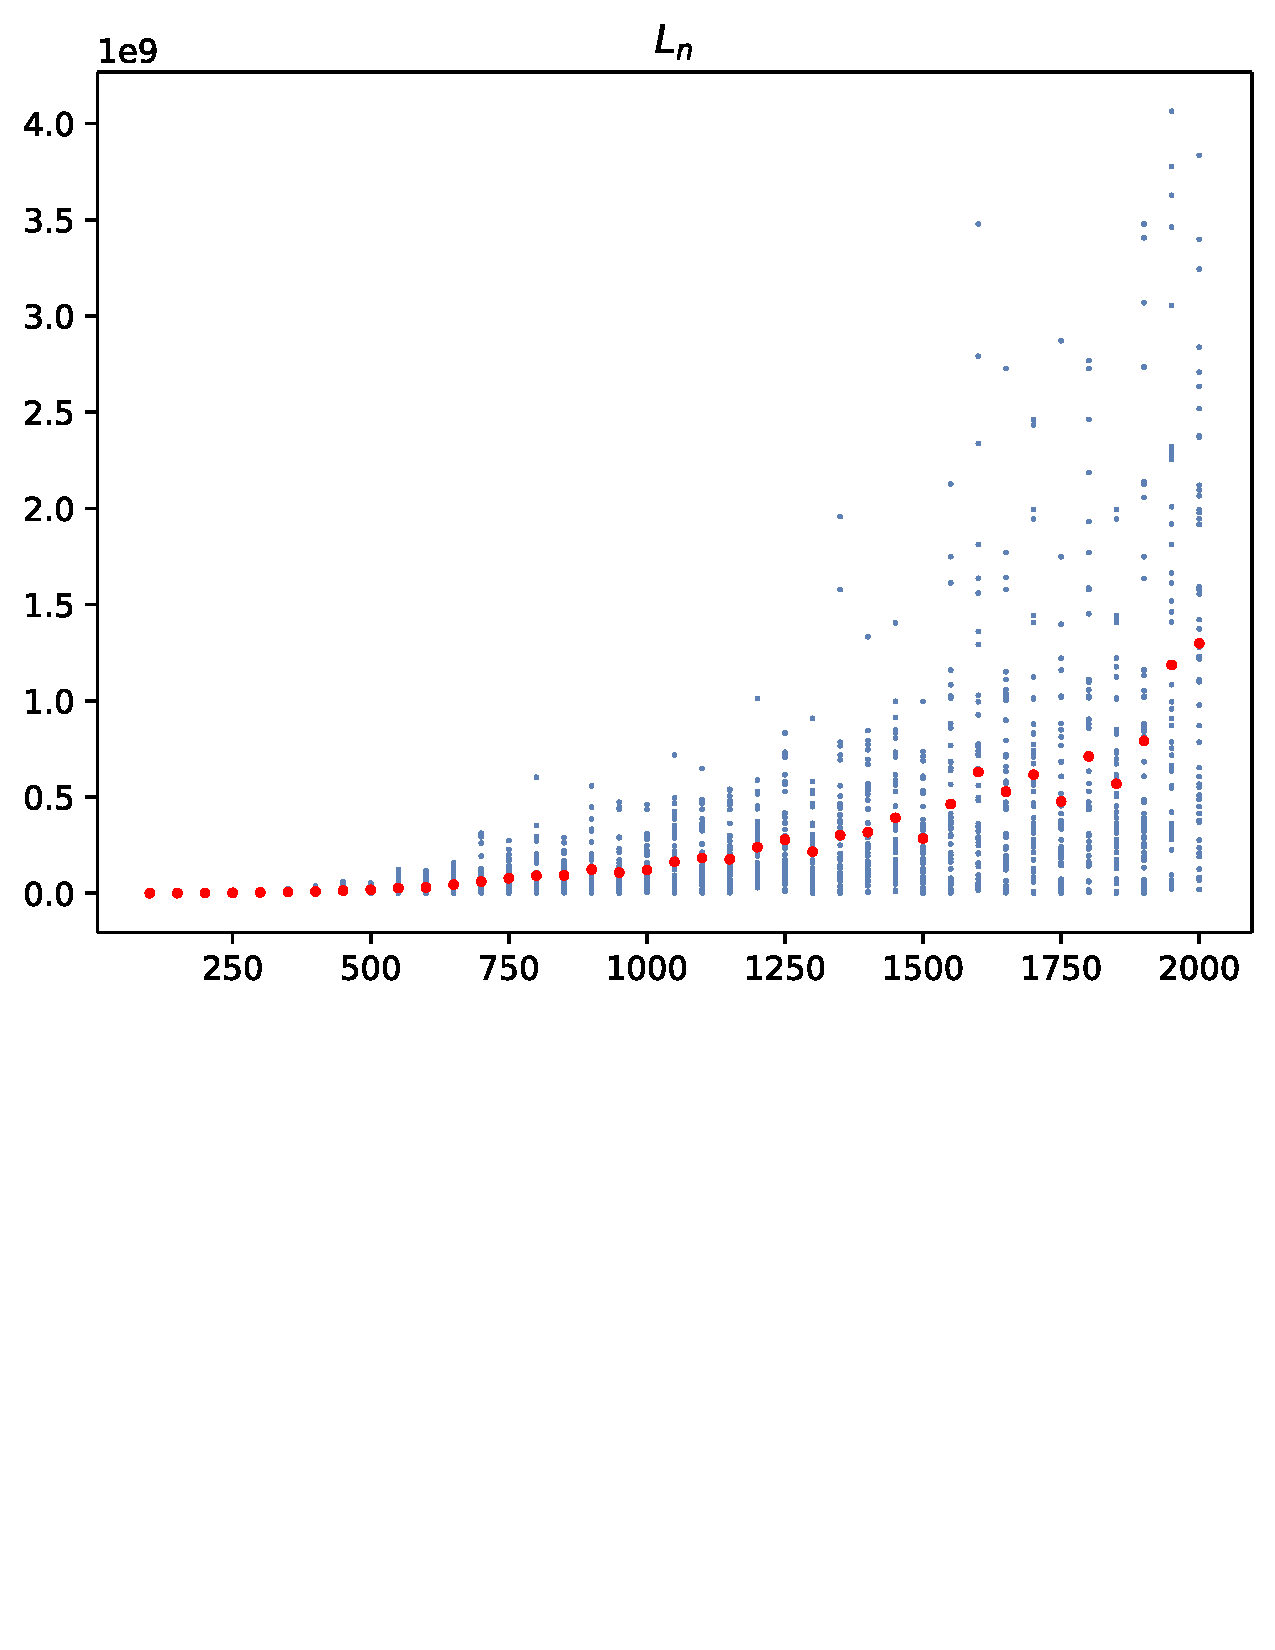
\includegraphics[width=12cm, trim = 0 11cm 0 0, clip]{images/e.pdf}
\end{figure}

\begin{figure}[H]
    \centering
    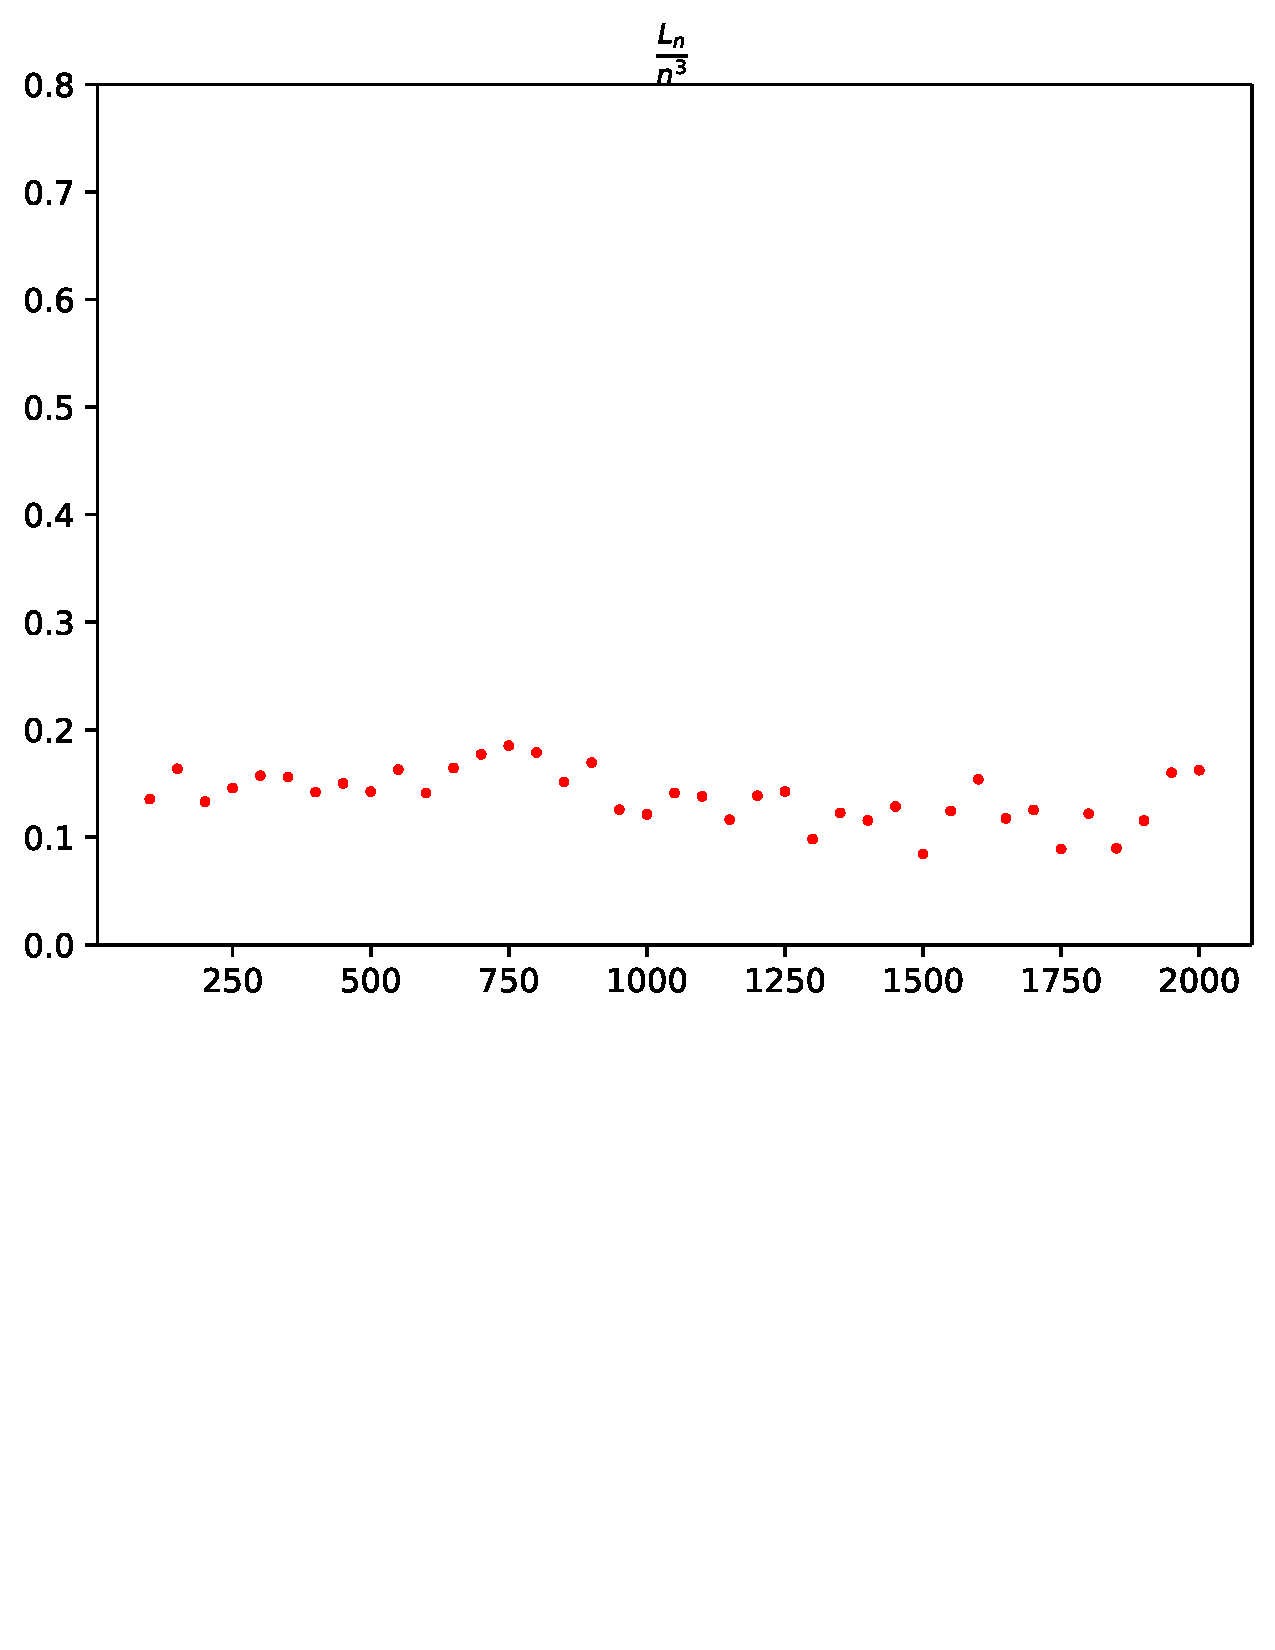
\includegraphics[width=12cm, trim = 0 11cm 0 0, clip]{images/e1.pdf}
\end{figure}

Dla wielkości $L_n$ już od początku widać bardzo szybki wzrost wartości. Na drugim wykresie widać, że
\[ L_n = \Theta (n^3) .\]

\section{Podsumowanie}

Dla każdej z wyznaczanych wielkości wraz ze wzrostem wielkości grafu rosła rozbieżność wyników dla poszczególnych prób. Mimo to dla (wybranego przeze mnie) $k=50$ asymptotyka była widoczna dla każdej ze statystyk.

\end{document}